%%% THIS IS THE TEMPLATE, MODIFIED FROM THE COMPUTER SCIENCE
%%% TEMPLATE OF THE UNIVERSITY OF HELSINKI
\documentclass[officiallayout]{tktla_modified}
%\documentclass[officiallayout,a4frame]{tktla}

%%%% ALL THE PACKAGES TO BE USED FOR THE DOCUMENT
\usepackage[latin1]{inputenc}
\usepackage{latexsym}
\usepackage{graphicx}
\usepackage[intoc]{nomencl}
\renewcommand{\nomname}{Abbreviations}
%\usepackage{etoolbox}
%\bibliographystyle{plainnat}
\usepackage[round]{natbib}
\bibliographystyle{chicago_2} %chicago 2 has 5 author max in Bib
\setlength{\bibsep}{0pt} %% set the separatio between the references
%\usepackage[nottoc]{tocbibind}
\usepackage[T1]{fontenc}
\usepackage{showframe} % just to show the alignment
%\usepackage{layout}   %% prints the layout of the page when is indicated
\let\cleardoublepage\clearpage %% delete the blank pages between sections
\usepackage{hyperref}
%%% can fine tune the margins of the book %%%%%%%%%%%%%%%%
\usepackage[
  left=0.7in, right=0.7in,
  bottom=0.75in,
  bindingoffset=0.25in,
  heightrounded,
]{geometry}
\usepackage{multicol}
%%% CONFIGURE THE BOXES %%%%%%%%%%%%%%%%%%%%%%%%%%%%%%%%%%
\usepackage[framemethod=TikZ]{mdframed}
\usepackage{fancyref}
\mdfdefinestyle{boxstyle}{ rightline=true,
innerleftmargin=10,innerrightmargin=10,frametitlerule=true,
frametitlerulecolor=red!15, backgroundcolor=red!15,frametitlerulewidth=2pt}


% Use adjustwidth environment to exceed column width (see example table in text)
\usepackage{changepage}
% rotating package for sideways tables
\usepackage[clockwise]{rotating}
%\usepackage[figuresleft]{rotating}
%%% change header and spacing of chapters %%%%%%%%%%%%%%%%%%
\usepackage{titlesec}
\titleformat{\chapter}[display] {\selectfont\huge\bfseries}{}{0pt}{\huge}
\titlespacing{\chapter}{0pt}{-40pt}{5pt}
\titlespacing*{name=\chapter,numberless}{0pt}{-10pt}{5pt}
%\titlespacing{\section}{0pt}{15pt}{5pt}
%\titlespacing{\subsection}{0pt}{10pt}{2pt}
%\titlespacing{\subsubsection}{0pt}{5pt}{0pt}

%% modify the itemize, without spaces and with roman numbers %%%%%%%%%%
\usepackage{enumitem}
\setlist{nosep} % or \setlist{noitemsep} to leave space around whole list
\renewcommand{\theenumi}{\roman{enumi}}

%%%%% remove the spacing before the nomenclature (not necessary after the titlespacing mod)
%\makeatletter
%\AtBeginEnvironment{thenomenclature}{%
%  \patchcmd{\@makeschapterhead}{\vspace*{50\p@}}{}{}{} }
%\makeatother
\usepackage{epigraph}
\usepackage[font={footnotesize},labelfont=bf]{caption}
%%%%%%%%%%%%%%%%%%%%%%%%%%%%%%%%%%%%%%%%%%%%%%%%%%%%%%%%%%%%%%%%%%%%%%%%%%%
%% ------Data to produce the front page ------------
\title{\hfill\break \hfill\break   %% 2 lines in blank (adding space)
Estimating complexity and adaptation 
%in space and time 
in the embryo:
\\ a statistical developmental biology approach
}
\author{Irepan Salvador-Mart\'inez}
\authorcontact{irepan_salvador@hotmail.com\par
  http://cs.helsinki.fi/John.Smith/}
\pubtime{November}{2016}
\reportno{0}
\isbnpaperback{000-00-0000-0}
\isbnpdf{000-00-0000-0}
\issn{1238-8645}
\printhouse{Unigrafia}
\pubpages{7} % --- remember to update this! 

% For article-based theses, the number of the last page of the list of
% references of the preamble part + the total number of the pages of
% the original articles and interleaf pages.

%% ------Data to produce the Supervisor/Custos ------------
\supervisorlist{Isaac Salazar-Ciudad, University of Helsinki, Finland}
\preexaminera{Pavel Tomancak, Max Planck Institute of Molecular Cell Biology and \par
              \quad\quad Genetics in Dresden, Germany}
\preexaminerb{Gregor Bucher, Georg-August-University G{\"o}ttingen, Germany}
\opponent{Johannes J{\"a}ger, Konrad Lorenz Institute, Austria}
\custos{Name, University, Country}

\thesiscommitteea{Jukka Jernvall, University of Helsinki}
\thesiscommitteeb{Osamu Shimmi, University of Helsinki}
\thesiscommitteec{Mikael Fortelius, University of Helsinki}


%\generalterms{thesis, example, another example, still more examples,
%  more and more examples}
%\additionalkeywords{example, an example phrase with many words}
%\crcshort{A.0, C.0.0}
%\crclong{
%\item[A.0] Example Category
%\item[C.0.0] Another Example
%}
\permissionnotice{
  To be presented in \ldots{} text of a long permission notice. Text of
  a long permission notice. Text of a long permission notice. Text of
  a long permission notice. Text of a long permission notice. Text of
  a long permission notice.
}

%\newtheorem{theorem}{Theorem}[chapter]
%\newenvironment{proof}{\noindent\textbf{Proof.} }{$\Box$}

%%%%%%%%%%%%%%%%%%%%%%%%%%%%%%%%%%%%%%%%%%%%%%%%%%%%%%%%%%%%%%%%%%%%%%%%%%%
%%%% -----------------------------------------------------------------
%%%% ----------------BEGIN OF THE DOCUMENT----------------------------

\begin{document}
%\layout					%%% here to print LAYOUT
\frontmatter

\maketitle
\makenomenclature
%\begin{abstract}
%\end{abstract}

\begin{acknowledgements}
  
\end{acknowledgements}

%%%%%%%%%%%%%%%%%%%%%%%%%%%%%%%%%%%%%%%%%%%%%%%%%%%%%%%%%%%%%%
%% reduces the space between lines in table of contents
\renewcommand{\baselinestretch}{0.75}\small
\tableofcontents
%% back to normal
\renewcommand{\baselinestretch}{1.0}\normalsize
%%%%%%%%%%%%%%%%%%%%%%%%%%%%%%%%%%%%%%%%%%%%%%%%%%%%%%%%%%%%%%%

\mainmatter

%%%% -----------------------------------------------------------------
%%%% ---------- BEGIN OF THE MAIN TEXT -------------------------------
%%%% -----------------------------------------------------------------

\pagenumbering{gobble}% Remove page numbers (and reset to 1)

\mychapter{0}{List of publications}

%%%% ---------ABREVIATIONS------------------------------------------
\printnomenclature

%%%% ---------- ABSTRACT---------------------------------------------

\mychapter{0}{Abstract}
	
Embryonic development has amazed scientists and philosophers for centuries.

Many reasons have been evoked for the perceivable complexity increase that transforms a single cell into a larva or an adult (even when complexity has eluded an unique definition).
Aristotle claimed a "vital force" guided embryogenesis. %Eventually, 
Vitalism was substituted by preformationism and epigenesis explanations in the 18th century.
%
Since the 1980's, when it became clear that genes play a key role in embryogenesis, 
%Nowadays, 
the causal mechanisms for such complexity increase are being searched for at the cellular and molecular level.

Using the number of cell types as complexity measure, its increase during development is self-evident: the embryo begins with one cell type (zygote) and concludes with up to 200 cell types (in mammals). 
This process can also be called embryo compartmentalization.
%From many discoveries since the 1980's, it has become clear that some genes play a key role in the embryo compartmentalization. 
At the level of gene expression, it its assumed that in early development, genes are initially expressed in large domains on the embryo. Then, at later stages, their expression become spatially restricted, until some genes are expressed in a cell-specific manner.
%
For many crucial developmental genes (e.g., Hox genes), the spatio-temporal expression dynamics, and how it relates to the embryo compartmentalization, has been thoroughly described.
It is not clear however, if the dynamics are similar for the rest of the genes deployed in development, or if there are differences between different types of genes.

-----------------------------

Adaptive reasons have been also said to be the cause for the increase in complexity.
A change during development would be adaptive if it increases the fitness of its bearer, even when the effect of this developmental change is realized until the adult or larva.
%The increase in complexity (or any change in development) has been considered for some authors as the adaptations of the embryo to its environment.

Many methods of molecular evolution estimate the action of natural selection based on the quasi-neutral evolution model.
Under this model, an adaptive change that has been caused by a genetic mutation, can be traced in the DNA sequence, as a positive selected site would show less variance than other sites evolving neutrally.

Recently, methods of population genomics use divergence ans polymorphism (inter-specific and intra-specific variation) to measure more precisely the proportion of adaptive mutation at the molecular level.

----------------------------
Importantly, if different developmental stages show distinct levels of positive selection or stabilizing selection,
some specific patterns, when comparing the development trajectories of different species in a group, might be recognizable.
% specific patterns might appear (patterns of what?) when comparing the divergence between different species.
Two related models currently under much discussion? are:
%This is related to already proposed models of divergence: 
1)von Baer's laws and the hourglass model.
The former states that the development of 2 species would be very similar in early stages and increasingly divergent in subsequent stages. In contrast, the latter states that development is less divergent at mid development.

%Such patterns could be due to selection or constrant..
%The print in natural selection on the genome is useful to discern between these scenarios.
%Some regarded each embryonic stage to have adaptation as the result of the constant interaction of the embryo with its environment (whether external or internal).
%Others have distinguished the adaptations in the embryo from those from the adult, stating that the former are product of internal selection, instead of being product of natural selection, as the latter.
------------------------------------------
In here, I will use gene expression information to estimate 
both complexity and adaptation in the embryo.

I will use a statistical approach, this means that no special emphasis on specific genes or pathways would be made. 
Instead, my intention is to provide a broad picture on the spatiotemporal change in complexity and adaptation in the embryo.

%I take advantage of available databases of gene expression.
%I analyze complexity using two popular developmental biology models: Drosophila melanogaster and Ciona intestinalis.
For the estimation of complexity, I analyzed gene expression data (from thousands of in situ hybridization experiments) of two popular developmental biology models: Drosophila melanogaster and Ciona intestinalis (from available databases) and developed quantitative measures of complexity.

To analyze adaptation, I combined the D. melanogaster transcriptomic data with genomic data from the DGRP project. With the DFE-alpha method (which uses coding-region polymorphism data and coding-region divergence between D. yakuba and D. melanogaster to estimate the proportion of adaptive changes), I chart a spatial map of adaptation of the fruit fly embryo's anatomy. 

Also, I analyze the pattern of positive selection through the entire life cycle of D. melanogaster.

Briefly, 

we found that low rates of adaptive change are found in the digestive system and high rates in the gonads and parts of the forming head. We also found that the regions that exhibit the highest rates of adaptation express, on average, genes that are phylogenetically young

%%%% -----------------------------------------------------------------

\chapter{Review of the literature}

\pagenumbering{arabic}% Remove page numbers (and reset to 1)

This work is based and uses concepts from three main biology fields: 
developmental biology, evolutionary biology and genetics.
Nowadays, the union of these scientific fields form multiple research programmes. 
Only in evolutionary developmental biology (evo-devo), the explicit union of the first two fields, at least four major research programmes have been recognized (Muller, 2006).
However, these fields have not always gotten along well. 
Some decades ago, there was a (CLEAR? CONCEPTUAL, EPISTEMOLOGICAL?) separation between evolutionary biology and developmental biology, even when embryology (which slowly transformed into developmental biology in the middle of the 20th century, see \citealp{Horder2010}) was considered crucial for the study of evolution in the 19th century.

In the following section, I will make a brief introduction of the scientific (and philosophical) origins of developmental biology, with special attention to its relations with evolutionary biology and genetics (for a comprehensive review on this issue, see: \citealp{amundson2005changing}; \citealp{gilbert1991conceptual}).
But before that, it might be useful to define what development is, so firstly, I will address this apparently simple question.

\subsection*{What is development?}
	\setlength{\epigraphrule}{0\p@}
\setlength{\epigraphwidth}{.7\textwidth}
\epigraph{\textit{" It is not enough to see that horse pulling a cart past
the window as the good working horse it is today; the picture
must also include the minute fertilised egg, the embryo in its
mother's womb, and the broken-down old nag it will eventually
become."}}{C. H. Waddington 1957}

It seems that there is no unique or straightforward answer to this question.
Sometimes, the study of development is implicitly considered to be the same as the the study of embryology \citep{Horder2010}.
%Traditionally, the problem of development has been studied by embryologists. However, embryonic development does not necessarily equate to development,
%theDevelopment is sometimes equate to embryonic development, probably due to the fact that developmental biology origins come from embryology.
%Equating embryonic development to development could be problematic 
This could be problematic when considering organisms with complex life cycles. For example, holometabolous insects, in addition to embryonic development, undergo a complete metamorphosis (from pupa to adult). This post-embryonic development shows clear similarities to its embryonic counterpart, specially in the imaginal disc pattern formation.%, a process that could be considered a second embryonic development.

Currently, the most common definition of development refers to the set of processes through which an egg is transformed into an adult \citep{Horder2010,Minelli2011}.
Already in 1880, Ernst Haeckel defined development in similar terms: "individual development, or the ontogenesis of every single organism, from the egg to the complete form is nothing but a growth attended by a series of diverging and progressive changes" \citep{haeckel_historycreation1880}.

Some authors criticize this egg-to-adult view to be an "adultocentric" view of development, and suggest instead to consider within the boundaries of development the whole life cycle of an organism \citep{Gilbert2011,Minelli2011}.
Julian S. Huxley and Gavin R. de Beer said that development "is not merely an affair of early stages; it continues, though usually at a diminishing rate, throughout life" \citep{huxley1963elements}.

%However, that this concept is not applicable to some organisms (Minelli in book). Some animals or plants instead of having an egg or seed stage as means of reproduction have buds or other vegetative parts.

%But even after considering the whole life cycle complications appear in cases in which the common notion of development of an individual organism would not apply, as in polyembryonic development or colonial organisms \citep{Minelli2011}.
There have been recent attempts to construct a broader concept of development \citep{Griesemer2014,Moczek2014,Pradeu2014} For example, Armin P. Moczek defines development as "the sum of all processes and interacting components that are required to allow organismal form and function, on all levels of biological organization, to come into being" \citep{Moczek2014}.
%
The main challenge on adopting a new concept of development which is more inclusive, is to maintain its intuitiveness and applicability in scientific research.

Throughout this dissertation I will use the "common view" of development \citep{Minelli2014}, that considers the egg and the adult as the start and end of individual development respectively.
%even when for practical reasons, some analysis of this dissertation (article 1 and 3) include only embryonic development. 
However, and mainly for practical reasons, the major part of the analyses presented here (sudies I-III) are restricted to embryonic development.

	
%\section{On the history of developmental biology}
%	\input{./Parts/Literature_DevBiol_History.tex}
	
%\section{On the statistical approach in Biology}
%	The statistical approach I have used in here, is nothing but new.

Darwin used a statistical approach to describe the action of natural selection (REF Darwin). For him, given the origination of small variations in natural populations, the occurrence of any advantageous variation in an individual, as slight it could be, would be reflected in a better chance of survival and to procreating their kind (Darwin). With many generations, the differential survival of the variants, would produce a change in the population mean. 
The effects of natural selection are thus only observable at the population level.

A more formal approach came from physics, more precisely from the study of diffusion of gases in the 19th century.

Against the main views of his contemporaries, which considered that all the particles in a gas move at the same speed, J. C. Maxwell proposed that each particle of a gas moved with different velocity and direction, both changing after the particles collision among them (REF Maxwell 1,2).
The velocities in all directions are distributed among the particles according to a certain law. As it was impossible to observe the behaviour of all the particles, their properties could only be described at a statistical level, as the average movement of large numbers of gas particles.

For Boltzmann and Gibbs, which extended the studies on gas diffusion, the study of large numbers was not only important to overcome the problem of not being able to study each individual particles, also because their individual behaviour is not interesting at all (Jacob, logic of life). Knowing the movement and direction of each particle would not give more information than the population as a whole.

After the success of statistical mechanics, its methodology expanded to many other scientific fields.
Laws could be applied to solve previously intractable problems by collecting sufficient information of a great number of cases of the same class and calculating its mean. The aim of the statistical approach is then to "obtain a law which transcends individual cases" (Jacob).

This novel approach changed biology drastically, transforming it into a quantitative science. As Fran\c{c}ois Jacob said, "at the end of the nineteenth century, the study of living beings was no longer a science of order, but one of measurement as well".


%	\clearpage 	
\section{Complexity}
	
The increase in complexity in an organism during embryogenesis is probably one of the most intuitive processes of animal development, 
even when there is no consensus definition of what exactly complexity is and how complexity should be measured.


A general definition could be "the number of component parts" of an organism.
These "parts" might be body segments (e.g., of an insect) or genes
	\citep{Arthur2010}.
It is evident that these definitions are problematic.
It is doubtful to say that some centipede is more complex than a beetle, just based in the different number of segments they have.
Also, it is already acknowledge that there is no relation between the number of coding-genes and morphological complexity.
This lack of correspondence, sometimes referred as the "G-value paradox"
	\citep{Hahn2002},
became evident with the release of the first eukaryotic genome sequences.
Decades before, the lack of correspondence between genome size and organism complexity (or "C-value paradox") was also noted.


An alternative definition of complexity includes not only the "number of parts" but also the "interaction among parts" 
	\citep{Arthur2010}.
This could be illustrated with the number of gene-gene interactions (e.g., expression regulation by a transcription factor binding to a promoter region of another gene),
such that when comparing two different organisms that have same number of genes, 
one organism could be considered to be more complex than the other if the former has more gene-gene interactions than the latter.
Again this definition is disputable, as it is acknowledged that during evolution gene-gene interactions (or gene regulatory network) underlying a phenotype
can increase their complexity without affecting the phenotype itself
	\citep{Muller1999,True2001,Salazar-Ciudad2009}.

\subsection{Complexity Increase in Evolution and Development}

The increase in complexity in evolution has has been a topic of interest for more than a century.
Early views of evolution saw the increase in complexity as inexorable, with all the species descending
from simpler ancestral forms and with the human species as the latest and more perfect product of 
the evolution of animals
	(REF Haeckel).
Recent views recognize that within a phylum complexity of the species can increase or decrease.

-parasites

-cave animals

-it is the range od complexity that increases


connection with development


	
\subsection{Complexity as number of cells}

A measure of morphological complexity that has been favoured by some authors (perhaps because of its intuitiveness), is the number of cell types that compose an organism 
	\citep{Bell1997,Bonner2004,McShea1996}.
Using the number of cell types as a proxy of morphological complexity, it can be said that during metazoan development, complexity increases as the zygote divides and differentiates into an adult with multiple cell types. This simple definition of complexity has its complications, as there are no clear-cut consensus criteria about how to define a cell type or about when a new cell type has arisen during development. 
However, even using this simple definition of complexity has its complications, as there is no clear criteria of how to define a cell type or how to determine when a new cell type has formed during development. It could be that at the morphological level a cell seems to be undifferentiated, but when isolating it, it differentiates in an autonomous way into a specific cell type, suggesting that the cell fate was already determined without the necessity of further interactions with other cells. 
In addition, this definition does not take into account that embryos do not only get more cell types, they also organize them in specific patterns in space that seem to increase in complexity over developmental time.

	
\subsection{Complexity at the molecular level}


At the level of gene expression it seems also clear that the embryo becomes progressively compartmentalized over time and space. In spite of this intuitiveness, there

%	\clearpage 
\section{Adaptation}
	Measuring adaptation is an important topic in evolutionary biology.

Since Darwin.. (REF Darwin)

In here, I refer to adaptation as a phenotypic character (or modification in a phenotypic character) that arise by natural selection in response to the environment, or other external factor.
Measuring adaptation at the phenotypic level requires a clear understanding of the function of the phenotypic character under study, and how the modification of this trait would affect the fitness of the bearer organism 
	\citep{EmiliaSantos2015}. 

Importantly, all phenotypic changes (whether a new character or a modification of an existing character) is produced from a change in development.
For example, the difference in the beak size and shape between the famous Galapagos Darwin's finches (REF Darwin), a classic example of adaptive change under natural selection, has been shown to be regulated by the differential expression of the genes CaM 
	\nomenclature{CaM}{Calmoduline}
and BMP4 
	\nomenclature{BMP4}{Bone morphogenetic protein 4}
during development. A proposed model for BMP4 and CaM role in beak size and shape explains both elongated and deep/wide beaks of these finches
	\citep{Abzhanov2006}.

So, even when natural selection acts in the adult phenotype (or in the larva, in the case of species with a feeding larva stage), we should be able to find changes in development that would explain an adaptive change in the adult or larva.


Some other remarkable examples of the genetic-developmental basis of adaptive change are:

-

-

It is evident at this point than many of the developmental changes leading to an adaptation are (at least partially) caused by mutations in gene regulatory or coding sequences.
Therefore, the effects of natural selection could be traceable looking at the adaptive changes in the genes expressed in different times and locations during development. There is an entire field within evolutionary biology, namely molecular evolution, dedicated to explain the sequence changes in molecules as DNA,
	\nomenclature{DNA}{Deoxyribonucleic acid}
RNA 
	\nomenclature{RNA}{Ribonucleic acid}
and proteins. 


\subsection{Molecular evolution}

The theoretical basis of the molecular evolution field includes concepts from evolutionary biology and population genetics. At the DNA level, any transmissible change in the sequence is considered a mutation. 
The most simple change is a point mutation or single nucleotide polymorphism (SNP),
\nomenclature{SNP}{Single nucleotide polymorphism} 
which is a change in a single nucleotide in the DNA sequence of a locus of two individuals. 
If the individuals belong to the same species, this mutation is referred as polymorphism. In contrast, divergence refers to the mutations when individuals from different species are taken into account. 
SNPs occur in non-coding and coding DNA sequence. A single point mutation that occurs in a coding sequence can be classified in two categories, depending on the effect of this mutation in the protein sequence: i) synonymous mutation and ii) non-synonymous mutation.
A synonymous mutation does not affect the amino-acid sequence of the protein, albeit it can affect its function 
	\citep{Kimchi-Sarfaty2007}
or the gene transcriptional efficiency (REF).
A non-synonymous mutation does affect the amino-acid sequence of the protein whether by changing a single amino-acid (missense mutation) or by producing a stop codon (non-sense mutation) which results in a truncated version of the protein.

As the non-synonymous mutations can affect dramatically the structure and function of the protein, it is expected that most of non-synonymous mutations would have a negative fitness effect.
However, it is also expected that a fraction of non-synonymous mutations, or adaptive substitutions, would have a positive fitness effect that (depending on the strength of the fitness effect) could lead to the fixation of that mutation in the population.

An important branch of the molecular evolution field is dedicated to the identification of adaptive substitutions in a species, which has lead to the development of many statistical tests. 
Importantly, these tests are based on the neutral theory of evolution, proposed by Kimura
	\citep{Kimura1968}.

\subsection{Neutral theory of evolution}
In 1968, Mooto Kimura calculated the average rate of nucleotide substitutions in the evolutionary history of mammals.
The result of his calculations was that, on average, one nucleotide has been substituted every 2 years.
For him, this very high rate of substitution was only explainable if most mutations were almost neutral in natural selection 
	\citep{Kimura1968}.
This was in contrast with the prevailing view at the time that practically no mutations are neutral (REF).
More importantly, the neutral theory provided a set of testable predictions, providing a null-hypothesis of molecular evolution.
This allowed the development of statistical methods to detect adaptive changes, i.e., we can say that a sequence has been under positive selection if the amount of changes exceeds the number of changes expected only by neutral evolution.
One of the most popular tests is the McDonald-Kreitman test (MKT),
	\nomenclature{MKT}{MacDonald-Kreitman test}
which estimates the proportion of the adaptive substitution resulted from natural selection.

\subsection{McDonald-Kreitman test}
John H. McDonald and Martin Kreitman developed this test in 1991 when analysing the divergence in the Adh 
	\nomenclature{Adh}{Alcohol dehydrogenase}
locus in three Drosophila species
	\citep{McDonald1991}.
The main assumption of the MKT is that the substitutions in a protein are neutral if the 
inter-specific ratio of non-synonymous (Dn) to synonymous (Ds) changes is equal to the 
intra-specific ratio of non-synonymous (Pn) to synonymous (Ps) changes (i.e. Dn/Ds = Pn/Ps).
Any departure from these equality would imply the action of positive or negative selection.
If some of the changes are result from positive selection, the ratio of non-synonymous to synonymous variation within species should be lower than the ratio of non-synonymous to synonymous variation between species (i.e. Dn/Ds > Pn/Ps). 
In the case that the observed ratio of non-synonymous to synonymous variation between species is lower than the ratio of non-synonymous to synonymous variation within species (i.e. Dn/Ds < Pn/Ps) 
then negative selection is at work.

Since mutations under positive selection spread through a population rapidly, they don't contribute to polymorphism but do have an effect on divergence.

Although the MKT has been proved robust to many sources of error (e.g., variation to mutation rate across the genome), it can underestimate the proportion of adaptive changes in the presence of slightly deleterious mutations
	 \citep{Messer2013,Eyre-Walker2006a}.
Recently, more sophisticated methods based on the MKT have been developed to correct for underestimation of adaptive evolution in the presence of slightly deleterious mutations. 


\subsection{Distribution of Fitness Effects}

To have a more precise estimate of the proportion of adaptive substitutions it is important to consider the relative contributions of the different types of mutations, based on their fitness effects.
Because even when for simplicity the mutation effects are usually classified in advantageous, neutral, and deleterious, there is actually a continuum of selective effects, from strongly deleterious, 
to highly adaptive mutations	
	\citep{Eyre-Walker2007},
with weakly deleterious, neutral and slightly adaptive mutations in between.

The relative frequencies of all these type of mutations is called the Distribution of Fitness Effects (DFE).
	\nomenclature{DFE}{Distribution of Fitness Effects}
The DFE has other practical implications, like predicting the effects on the genetic variation in a population with low population size.
In order to know the DFE, a few experimental approaches exist. The most direct method is whether to induce 
	\citep{Sanjuan2004}
or to collect
	\citep{MUKAI1964}
spontaneous mutations and assay their effects (fitness) in the laboratory.
As can be expected, this experiments require many generations to gather sufficient data, so these approaches have been used mainly in micro organisms
	\citep{Eyre-Walker2007}.
A caveat of these experimental approaches is that, in order to identify the effect of a mutation, its effect has to be detectable in a fitness assay.
Therefore, these methods give valuable information for mutations with relatively large effects.

An alternative approach is to infer the DFE by analysing patterns of DNA sequence differences at intra and inter-specific level (polymorphism and divergence respectively).
The methods using this approach rely mainly on two assumptions:
i) the probability that a mutation spreads to a certain freq in a population (or to fixation) depends on the strength of selection (positive or negative) acting on it.
Severely deleterious mutations have lower probability to reach a high frequency in a population.
ii) the efficiency of selection depends on the effective population size. 
With a high effective population size, selection is more efficient and a smaller proportion of mutation will behave as effectively neutral.

The "absolute strength" of selection on a mutation is then measured as $N_{e}s$, the product of the effective population size ($N_{e}$)
	\nomenclature{$N_{e}$}{Effective population size}
by the selection coefficient ($s$)
	\nomenclature{$s$}{Selection coefficient}
of the mutation. Mutations with $N_{e}s$ much less than 1 are effectively neutral, while $N_{e}s$ greater than 100 have no chance to appear as polymorphism.

\subsection{DFE-alpha}

Eyre-Walker and collaborators 
	\citep{Eyre-Walker2009}
proposed a method to estimate both the DFE and the proportion of adaptive nucleotide substitutions ($\alpha$)
	\nomenclature{$\alpha$}{Proportion of adaptive nucleotide substitutions}
using polymorphism and divergence data.
More specifically, they use the polymorphism site frequency spectrum (SFS) 
	\nomenclature{SFS}{Site Frequency Spectrum}
to estimate the DFE and then use this estimated DFE to estimate the proportion of substitutions under positive selection between species.
This method, assumes that there are two types of nucleotide sites: 
i) sites at which all mutations are neutral and ii) sites at which some of the mutations are subject to selection (positive or negative).
Also it is assumed that any new adaptive mutation in a population would not be detected in the polymorphic phase but only in the divergent one, 
and that the DFE can be represented with a gamma distribution.
The advantage of using a gamma distribution is that very different distributions (e.g., normal, exponential, leptokurtic) can be represented using only a shape parameter and the mean of the distribution (Figure \ref{fig:Gamma}).

\begin{figure}[h]
  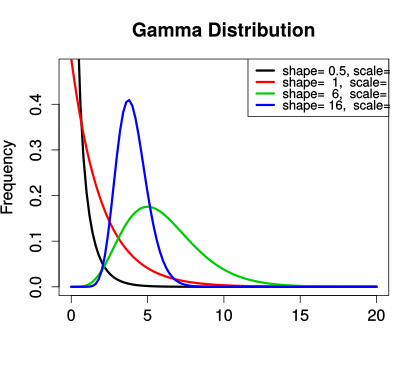
\includegraphics[width=7cm]{./Images/Gamma_dist.jpeg}
  \centering
  \caption{Example of different Distribution of Fitness Effects (DFE) represented by a gamma distribution.
  Many distributions can be represented by modifying the shape parameter of a gamma distribution, from
  a leptokurtic (shape parameter less than 1) to an exponential (shape parameter equal to 1) or a
  skewed normal distribution (shape  greater than 1).
   }
  \label{fig:Gamma}
\end{figure}


The divergence at the neutral sites is then proportional to the mutation rate per site and the predicted divergence at the selected sites, in the absence of advantageous mutations, 
is proportional to the product of the mutation rate and the average fixation probability of a selected mutation, 
which is inferred based on the DFE and other parameters estimated from the polymorphism data analysis
	\citep{Eyre-Walker2009}.
The difference between the observed and predicted divergences therefore estimates the divergence due to adaptive substitutions.

Using this method Eyre-Walker and collaborators 
In Drosophila genes, we estimate
that approximately 50\% of amino acid substitutions and approximately 20\% of substitutions in introns are adaptive
	\citep{Eyre-Walker2009}.

Molecular evolution simulations have been performed to test if the estimates of different tests, like the MKT and the more sophisticated DFE-alpha, are accurate under different realistic gene-structure and selection scenarios
	\citep{Messer2013}.
More specifically, the authors wanted to test how accurate these methods are in presence of genetic draft (stochastic effects generated by recurrent selective sweeps at closely linked sites)
and background selection (interference among linked sites by lightly deleterious polymorphisms).

They found that in the presence of slightly deleterious mutations, MKT estimates of $\alpha$ are severely underestimated.
They also found that the DFE-alpha is very accurate to calculate alpha when changes is demography are considered
	\citep{Messer2013}.
.




%	\clearpage
\section{Drosophila}
	


\subsection{Subsection one}


\subsubsection{Subsubsection one}


%	\clearpage
\section{The Hourglass model in \textit{Drosophila} }
	
%
%\subsubsection{Adaptation in the embryo}
%
%Usually, the study of adaptation
%- general considerations of adaptation in the embryo
%
%- example from marine animals
%- Whyte
%- entrenchment
%- adaptive changes that influence adult/larva characters
%- measurements of adaptation in the embryo in drosophila
%- heatshock, developmental time, Dn/Ds.. etc.
%\subsubsection{Hourglass model}

%%% von Baer vs Hourglass
\label{hourglass}

As I described briefly in section \ref{vonBaer}, von Baer stated in his "laws" that within a group of animals the general characteristics appear earlier in development, while the most special appear in late development \citep{vonBaer1828uber}.
%although he recognized that the early stages were different (Gilbert 2010)
This would lead to low morphological variation at early development, gradually increasing as development proceeds.

Other authors \citep{Medawar1954,Slack1993,Duboule1994,Raff1996} proposed an alternative pattern in which there is great variation in early and late development, while the mid-development would show less variation.
This pattern of variation (or conservation) has been called `phylotypic egg-timer' \citep{Duboule1994} and `developmental hourglass' \citep{Raff1996}.

% hourglass background
Duboule's concept of `phylotypic egg-timer' was based in the concept of `phylotypic stage' of \citet{Sander1983}, who coined this term to describe the convergence into a conserved segmented germ band stage in insects from very divergent early development \citep{Sander1996}.
In vertebrates, there has been controversy around what should be the phylotypic stage \citep{Ballard1981,Slack1993,Duboule1994}. \citet{Richardson1995} argued that indeed there is no single conserved stage in vertebrate's development and instead he proposed the term `phylotypic period' instead.

Initially, two explanations for the hourglass model were proposed.
Denis Duboule, after observing that the expression of the Hox genes seemed to coincide with the phylotypic stage, he considered that this could not be a coincidence and proposed that the activation of the Hox genes was the cause for the morphological invariance \citep{Duboule1994}.
In contrast, Rudolf A. Raff proposed that the phylotypic stage was the result of complex interaction between developmental modules at this stage  \citep{Raff1996}.

There is an ongoing discussion about whether the hourglass model (HG), the von Baer law
or some other pattern fits the divergence among developmental stages in phylogeny \citep{Richardson1997,Poe2004,Kalinka2012}.
	\nomenclature{HG}{Hourglass model}

Also, it is not clear if the HG, that seems to fit well in vertebrates and arthropods, would apply to other phyla \citep{Raff1996} \citep{Salazar-Ciudad2010}.
\citet{Salazar-Ciudad2010} has proposed that different patterns of variation throughout development in metazoan groups would correlate with different developmental types (a classification based on the relative use of signalling and morphogenetic events).

%% genetic hourglass
Recently, the HG have received support from different gene expression studies.
%Kalinka
\citet{Kalinka2010} used micro-arrays for six Drosophila species and quantified expression divergence at different developmental stages. They found that gene expression was most conserved during the extended germ-band stage (considered the phylotypic period) and that the non-synonymous divergence per site ($Dn$) correlated with their divergence measures.

They also showed that most genes fit best to models incorporating stabilizing selection and proposed that natural selection acts to conserve patterns of gene expression during mid-embryogenesis \citep{Kalinka2010}.

%Domazet & piasecka
The HG seems also to be reflected in the age of the transcriptome (mid-embryonic stage shows the older transcriptome; \citealp{Domazet-Loso2010}) and in the conservation of the regulatory regions (most conserved for genes expressed in mid-development; \citealp{Piasecka2013}).

%other based on DNA conservation
Studies measuring the conservation of genes at the DNA sequence level also seem to support the HG.
\citet{Davis2005} assessed whether proteins expressed at different times during \textit{D.  melanogaster} development varied systematically in their rates of evolution (comparing with \textit{D. pseudoobscura}) and found that proteins expressed early in development and particularly during mid-late embryonic development evolve slower.  
This suggests, according to the authors, that embryonic stages from 12 to 22 hours are
highly conserved between \textit{D. melanogaster} and \textit{D. pseudoobscura}, which is consistent with the HG.
%
In a similar study, \citet{Mensch2013} calculated the dN/dS ratio for more than 2,000 genes among six \textit{Drosophila} species, separating genes in three categories: maternal genes (genes whose products are left by the mother in the egg), genes expressed in early development and genes expressed in late development. They found that maternal genes and lately expressed zygotic genes show higher dN/dS ratios (i.e., are less conserved) than early expressed zygotic genes.
Finally, it has also been found that genes expressed in the adult have higher dN/dS ratios than genes expressed in the pupa and those of the pupa have higher dN/dS ratios that those expressed in the embryo \citep{Artieri2009}.

Some limitations of these last studies is that they classify the genes in a few broad temporal categories that do not permit to precisely determine the temporal dynamics of conservation and that are based only in divergence data (dN/dS ratios between two species).
A study that integrates polymorphism data from natural populations would improve the evolutionary interpretation of these patterns, as it would allow to estimate what proportion of the dN are adaptive (as explained in section \ref{alpha}).
Measuring adaptation is specially relevant as some authors have argued that the HG is caused by different selection pressures in early and late development \citep{Slack1993,Kalinka2012,Wray2000}

%%inter phyla comparison

%Recently, a study reported an inverted hourglass pattern
%(i.e., early and late conservation and mid-development divergence) when comparing developmental transcriptomes of ten different species, each from a different phyla [21](REF).
%	\clearpage
\section{Ciona}
	\subsection{Ciona as a model}
	The ascidian \textit{Ciona intestinalis}, a marine invertebrate animal, has a long history in developmental biology and evoutionary biology. 
	Darwin highlighted the importance of the ascidians due to their  close phylogenetic relationship to the vertebrates (REF). 
	Also, it provided one of the first evidences of localized determinants of cell specification \citep{Conklin1905}. 
	Although their adult form is a sessile filter feeder, its tadpole larva has characteristic features of the chordate group: a dorsal neural tube, a notochord surrounded by muscle and a ventral endodermal strand (Satoh, 1994).
	Ascidians show morphogenetic movements during gastrulation and neurulation similar to vertebrates and both share common genetic regulators of cell specification (REF).
	Their relative short life cycle, almost transparent body and rapid development facilitate many genetic techniques and are partly responsible for the re-emergence of \textit{C. intestinalis} as model organism in developmental biology \citep{Levin2012}.
	
\subsection{Current knowledge about Ciona development}
	The sequencing of the \textit{C. intestinalis} genome \citep{Dehal2002} facilitated its comparison with other vertebrate sequenced genomes and the analysis of gene expression through its life cycle.
	The \textit{C. intestinalis} genome is only 160Mb and contains ~16,000 genes, a gene number similar to the invertebrate \textit{D. melanogaster} genome and only is half of the genes found in some vertebrates (REF).
	This low number of genes (compared to vertebrates) can be explained by the finding that many gene families or subfamilies have only one representative in \textit{C. intestinalis} \citep{Dehal2002}.
	Relevant efforts have been made to describe the spatial expression patterns of individual genes (REF).
	The spatial expression patterns of  >1,000 cDNA clones have been described using whole-mount in situ hybridization techniques at different developmental stages \citep{Imai2004}.
	 Importantly, the developmental stages included cover a wide temporal range, e.g., blastula, gastrula and tapole stages (REF).
	 Taking advantage of the ascidian invariant cleavage pattern and well described lineage analysis \citep{Conklin1905,Nishida1987}, the spatial expression of many genes have been described at the single cell level up to the early gastrula stage (REF), making this an invaluable resource to investigate the spatio-temporal dynamics of gene expression.


	\clearpage
%%%% -----------------------------------------------------------------
%%%% -----------------------------------------------------------------

\chapter{Aims of the study}
\vspace{1cm}
In this work, I have analysed publicly accessible spatio-temporal gene expression data of two model organisms, \textit{Drosophila melanogaster} and \textit{Ciona intestinalis}, together with population genomics data of \textit{D. melanogaster}.
Using a statistical approach, I address these following questions, which have been selected for the great interest they have aroused in the scientific community since the early days of developmental and evolutionary biology:

\vspace{1cm}
%%%%%%%%%%%%%%%%%%%%%%%%%%%%%%%%%%%%%%%%%%%%%%%%%%%%%%%%%%%%%%%%%%%%%%%%%%
\begin{enumerate}[label=\Roman*]

\item How do complexity and compartmentalization increase in the embryo during development?
\vspace{0.5cm}

\item Are there differences in the pattern of compartmentalization and complexity increase when comparing different species (i.e., \textit{D. melanogaster} and \textit{C. intestinalis})?
\vspace{0.5cm}

\item Can adaptation be found in specific anatomical parts of the embryo or developmental stages? 
\vspace{0.5cm}

\item Is the Hourglass model supported by evidence of natural selection when considering inter and intra-specific variation at the DNA sequence level?

\end{enumerate}
%%%%%%%%%%%%%%%%%%%%%%%%%%%%%%%%%%%%%%%%%%%%%%%%%%%%%%%%%%%%%%%%%%%%%%%%%%
\vspace{1cm}

%
%These questions have been selected for the great interest they have aroused in the scientific community since the early days of developmental and evolutionary biology.
%%
%The work presented here is based on and uses concepts from three main biology fields: 
%developmental biology, evolutionary biology and population genetics.
%Nowadays, the combination of these scientific fields constitute multiple research programmes. Modern evolutionary developmental biology (evo-devo) is the explicit combination of the first two fields.
%	\nomenclature{evo-devo}{Evolutionary developmental biology}


%%%% -----------------------------------------------------------------
%%%% -----------------------------------------------------------------

\chapter{Material and Methods}
	\section{On the complexity measures used in this work}
	
In the following paragraphs I will describe the three measures of complexity I used in here: relative area/volume, disparity and roughness. I consider them complexity measures because they inform about specific features in embryonic development that are intuitively associated to the increasing complexity of the organism. The relative area/volume of expression relates to the notion of the progressive compartmentalization of the embryo, disparity informs about how the different parts of the embryo become more different (at the genetic level) from each other, and the roughness measure relates to the notion of genes being expressed in progressively more complex spatial expression patterns (as defined by the shape of the gene expression pattern).  For information on the statistical tests used (e.g., Kruskal Wallis, ANOVA, permutation test) see the corresponding study.


\subsubsection{Compartmentalization}

As mentioned before, the process of embryo compartmentalization, is expected to be largely reflected in the expression of the genes in progressively smaller areas. Therefore, a good measure of compartmentalization would be to measure the relative area of expression of all genes during development.
Gene expression patterns are usually visualized as 2D images, which reflect the distribution of a gene product from a specific anatomical view (e.g., lateral, dorsal).  Recently, methods like 3D imaging technique Optical Projection Tomography  \citep{Sharpe2003,Summerhurst2008} allow to record gene expression patterns in 3D.
%
In the case of 2D images, the measure of compartmentalization I use in here is the relative area of the expression, i.e., the pixels with expression divided by all the pixels of the embryo image. This "relative area" measure ranges from 0 (no expression) to 1 (ubiquitous expression). 
In the case of a gene expression in 3D, the compartmentalization measure becomes the relative volume of expression, which also ranges from 0 to 1 and is calculated as the volume of the cells/tissues with expression divided by the whole embryo volume.
%Of course it could be said that the compartmentalization of an embryo should not only be reflected in the decrease of the relative area of expression of the genes during development, but also should be reflected in a greater proportion of genes expressed differentially in different parts of the embryo. To account for this, I used a "disparity" measure (explained below), that would be informative in the mean degree of dissimilarity between the different parts of the embryo.

\subsubsection{Disparity}

The disparity measure is related to  McShea's "number of part types" complexity measure. Ideally, the number of cell types, if this could be precisely known, would be a good measure of complexity during development. However, as mentioned before, there is no clear criteria to determine when (at the genetic level) a new cell type is formed during development.
%
%Usually, genetic markers are used to determine if a cell (or its descendants) can be considered a specific cell type. This could be the case of anterior or posterior compartment cells within \textit{D. melanogaster} para-segments. For example, the use of wingless (\textit{wg}) or sonic hedgehog (\textit{hh}) in situ hybridization can be used to define if a cell is part of the anterior or posterior compartment. It could be said, however, that the earliest presence of expression of these genes marks the \textit{fate} of the cell, more than the actual cell type. In fact, before the anterior and posterior segment compartments are completely defined, the expression level of these genes changes over time and form a positive feedback to stabilize each other expression. Therefore, a cell that early expresses \textit{wg} would not necessarily differentiate into a posterior compartment if its neighbour para-segment does not express \textit{hh} \citep{Bejsovec1991}.
%
Instead of trying to determine the number of cell types during development, I decided to quantify how different at the gene expression level are the cells or regions in the embryo. In \textit{D. melanogaster}, as it was not possible to have expression for each individual cell, I divided the 2D embryo in "regions" of approximately the same area using polar coordinates (Fig. \ref{fig:roughness_regions}A; see study I). 
In the case of \textit{C. intestinalis}, I used expression data at a single cell level for the early stages and at tissue level for the tailbud stages (see study II).

To quantify this, I decided to use pearson's correlation as similarity measure between cells/tissues or regions. With this method, the expression of all the genes available in two cells can be compared, giving a value of 1 if all genes have exactly the same expression (their expression is completely correlated), to -1 if all the genes show opposite gene expression (their expression is anti-correlated). 
An advantage of this method is the possibility to include the information of all available genes, diminishing a possible bias in the gene selection. 
%
%The pearson's correlation matrix is a measure of gene expression similarity between genes. 
I computed pairwise similarities between cells/regions as the Pearson correlations using the function \textit{corSimMat} of the R package \textit{apcluster} \citep{Bodenhofer2011}. In here, I was interested on quantifying the difference (i.e., disparity) in gene expression between cells, not on their similarity. Therefore, the disparity between two cells becomes: disparity = 1 - pearson's similarity. The disparity measure ranges from 0 to 2, with a 0 value when the gene expression between cells is exactly the same.

\paragraph{Synexpression Territories} 
%Another advantage of using a Pearson's correlation matrix, is the possibility of using a clustering algorithm (e.g., hierarchical clustering). This has been used, for example, to find the main temporal patterns of gene expression in microarray analysis \citep{Eisen1998,Wen1998}.

Using the Pearson's similarity matrix I performed a hierarchical clustering of cells/ regions using the function \textit{hclust} of the R package \textit{stats} \citep{RCoreTeam2014} with the average method UPGMA and an euclidean distance function. The resulting dendrograms, with as many terminal branches as cell/regions analysed, were cut into a given number of clusters, called in here "synexpression territories".
In \textit{D. melanogaster} (study I and III) the dendrogram resulting from the analysis of the regions of all stages was cut into 40 synexpression territories. The territories are not exactly the same between study I and III, as in study III the clustering was done again with the 1199 genes dataset (see section \ref{insitu_drosophila}).
In \textit{C. intestinalis} (study II), because the information in the early stages is at the cell level while in the tailbud is at the tissue level, we performed two separate synexpression territory analyses one with the 32, 64 and 112 cells stages (n = 1550 genes), and another one with the early, mid and late tailbud stages (n = 820 genes).
The dendrograms resulting from the early and tailbud stages were cut in 24 and 10 "synexpression territories".

%Also, this method can be used to separate cell types based on the genetic differences between them \citep{gohlmann2009gene}.
%\textbf{AQUI PONER LOS TERRITORIOS DE CIONA Y DROSOPHILA}

%%%%%%%%%%%%%%%%%%%%%%%%%%%%%%%%%%%%%%%%%%%%%%%%%%%%%%%%%%%%%%%%%%%%%%%%%%%%%%%%%%%%%%
\begin{figure}[h]
  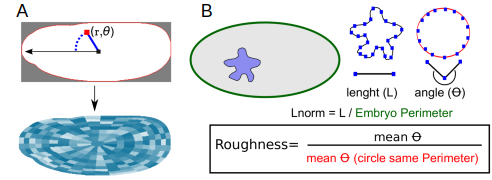
\includegraphics[width=0.75\textwidth]{./Images/roughness_regions.png}
  \centering
  \caption{\textbf{Polar regions and 2D roughness measure}. A) The embryo of each stage was divided in 257 regions using polar coordinates. The embryo for stage 11-12 is shown with the 257 regions in a random color. B) A schematic embryo (gray) with a gene expression pattern in blue. Roughness is the mean major angle ($\theta$) between each node (at every L length pixels in the contour) and its two immediate neighbours, normalized by the mean angle of a circle of the same perimeter. Image modified from Study I, reused with permission of Elsevier.
   }
  \label{fig:roughness_regions}
\end{figure}
%%%%%%%%%%%%%%%%%%%%%%%%%%%%%%%%%%%%%%%%%%%%%%%%%%%%%%%%%%%%%%%%%%%%%%%%%%%%%%%%%%%%%

\subsubsection{Roughness}
\label{Methods_roughness}
The roughness measure analyses the complexity of the shape of a gene expression pattern. In the case of 2D images, the shape of the gene expression pattern is extracted as a closed outline formed by the boundaries of gene expression. For 3D patterns, the shape of the expression pattern is the 3D external surface of the union of the cells that are expressing such gene.

Therefore, a gene expression pattern reflects necessarily the spatial distribution of the cells expressing such gene. When analysing and comparing the shape of diverse gene expression patterns, i.e., the cells/tissues with expression are different between genes, there is an obvious impossibility to determine landmark points (whether around a 2D outline or 3D surface) that would establish a clear one-to-one correspondence between them. This could be done in the case of comparing the expression pattern of a single gene at a specific developmental stage between different individuals.
Therefore, a landmark-free method (like outline methods for 2D or surface methods for 3D data) is best suited to deal with the type of data analysed in here.

There are practically no studies in the literature that have quantified and compared the shape of gene expression patterns in a systematic manner (one exception is the recent study of \citealp{Martinez-Abadias2016}). In here, I will consider that a gene expression pattern is complex based on the curvature of its 2D contour or 3D surface.

\paragraph{2D Roughness}
For 2D gene expression patterns, I used a "roughness measure", that is similar to the shape function $\phi^{*}(l)$ used in eigenshape analyses \citep{Lohmann1983}, as it measures how much the curvature of a closed outline deviates from the angles of a circle of the same perimeter (Fig. \ref{fig:roughness_regions}B; see study I). 
To calculate the roughness of a expression pattern I first selected points in the contour every L (length) pixels. Then, vectors between each node and the two immediate neighbour nodes in the contour are calculated and the biggest angle formed between them is measured. The roughness value is then the mean angle normalized by the mean angle of a circle of the same perimeter.

I selected the roughness measure instead of some other measure outline based method like Fourier analysis because the roughness value gives an intuitive descriptor of complexity, i.e., a value of 1 would be a simple "circle-like" shape, and a value greater than 1 would mean a higher curvature of the outline. \citet{McLellan1998} compared various measures of spatial complexity applied to the outlines of the leaves of many tree species. They included a "margin roughness" measure that is very similar to the one I use here (the difference is that they does not normalize by the mean angle of the circle nor he uses different lengths of vectors) and found that there was no marked differences between the margin roughness and a Fourier analysis with up to 64 harmonics (both performed equally well).
%On the contrary, one advantage of the Fourier analysis would be that it is an information preserving algorithm \citep{Pavlidis1980} i.e., it is possible to reconstruct the shape after the analysis, a feature that was not considered relevant for this study. 
Other feature of the roughness measure is that allows to measure the complexity of shape at different spatial scales (varying the L length). 
%Therefore, it can be tested not only if the complexity of the gene expression shape increases during development, also if this increase is the same at different spatial scales.

\paragraph{Dirichlet Normal Energy (DNE)}
	\nomenclature{DNE}{Dirichlet Normal Energy}
In order to use a similar measure of curvature in 3D, I used the Dirichlet normal energy (DNE; described briefly in section \ref{DNE_explanation}) which quantifies the deviation of a surface from being planar (Fig. \ref{fig:DNE}; see study II). 
Importantly, both measures are normalized to remove size and orientation effects.

%%%%%%%%%%%%%%%%%%%%%%%%%%%%%%%%%%%%%%%%%%%%%%%%%%%%%%%%%%%%%%%%%%%%%%%%%%%%%%%%%%%%%%
\begin{figure}[h]
  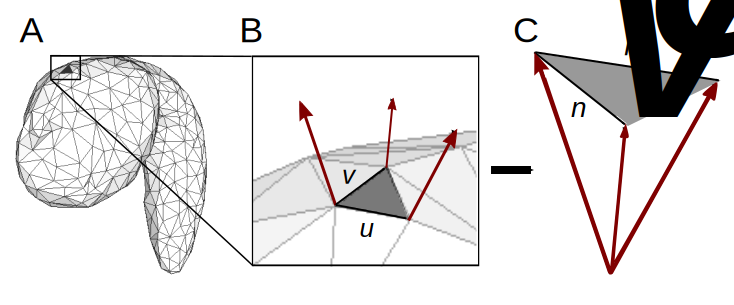
\includegraphics[width=0.6\textwidth]{./Images/DNE.png}
  \centering
  \caption{\textbf{Dirichlet Normal Energy (DNE).} A) A surface mesh representing a a mid-tailbud embryo in \textit{C. intestinalis}. B) DNE calculates the energy value $e(p)$ of each polygon (like the one in grey) in the surface. The polygon is characterized by vectors $u$ and $v$, which represent the edges of the polygon. Then, normal unit vectors are estimated as the normalized average of normal vectors of the triangle faces adjacent to each vertex (red arrows). C) If vertex normals are translated to a common origin point, their end points form a polygon with edge vectors $nu$ and $nv$, which represent the spreading of $nu$ and $nv$. In a simplistic way, DNE can be defined as the spreading of $nu$ and $nv$ relative to the spreading of $u$ and $v$  \citep{Bunn2011,Winchester2016}.
 }
  \label{fig:DNE}
\end{figure}
%%%%%%%%%%%%%%%%%%%%%%%%%%%%%%%%%%%%%%%%%%%%%%%%%%%%%%%%%%%%%%%%%%%%%%%%%%%%%%%%%%%%%

To calculate the DNE, I used the Morphotester software version 1.1.2 \citep{Winchester2016}
available in the webpage "http://morphotester.apotropa.com/". For details see study II.

It is important to mention that the aim of this analysis is not to discern which mechanisms (e.g., cell-cell signalling or morphogenetic movements) are responsible for the changes in complexity of the shape of gene expression pattern, but to quantify how this happens during embryonic development.

\subsubsection{The relationship between these measures}
\label{measures_relations}

The three different measures of complexity are informative of different and independent aspects of complexity and are not necessarily correlated. 
For example, a decrease in the area/volume of gene expression should not necessarily mean an increase in disparity, as the genes that are reducing their expression area could be restricted to the same part of the developing embryo. 
Only in the case of an embryo with all genes showing ubiquitous expression, there is a clear relationship between disparity and relative area/volume, as the relative area of expression and disparity would be 0 and 1 respectively. If there are however, many genes expressed in only a part of the embryo, these measures are not necessarily correlated. 

This can be illustrated with a simple example shown in Fig. \ref{fig:measures_relations}, in which there are different alternative gene expression scenarios of an imaginary embryo with six cells. In each scenario, the embryo expresses four genes in different relative areas (i.e., in a different number of cells). The mean relative area is 0.5 for all scenarios, but the mean disparity varies in a two-fold manner. In the scenario that shows the largest disparity, each cell expresses a unique combination of genes, while the scenario with the lowest disparity, 4 of 6 cells do not have a unique expression profile.

The roughness and disparity independence can be easily exemplified in the case of a blastula. Blastula is the name to define the multicellular aggregate stage that results from the subdivision (cleavage) of the zygote. The blastula shape topology and geometry is usually simple \citep{Forgacs_Newman2005}, typically consisting of a ball of cells with an interior cavity (called "blastocoel"). If in a spheric blastula, composed of also spheric cells (like that of a sea urchin) a large proportion of genes would be expressed ubiquitously and a small proportion of genes would be expressed in single cells, both roughness and disparity would be relatively low.
However in the case of a large proportion of genes expressed in different single cells, and a low proportion of genes expressed ubiquitously, the disparity would be high, but the roughness would be very similar than in the previous case. This would be because the roughness quantifies the shape of the expression pattern, irrespective to size. Therefore the roughness of a gene expression in a single spheric cell would be practically the same that the roughness of a gene expression in the whole spheric embryo.

The independence of the roughness measure with the size of the gene expression (i.e., relative area/expression) comes from the roughness normalization. The normalization of the 2D roughness consists of dividing the mean angle of a gene expression pattern by the mean angle of a circle with the same perimeter, and in the case of 3D roughness (i.e., DNE) it consists on transforming the 3D expression surface into a polygonal surface mesh with a determined number of polygons. 
%Therefore, these three measures of complexity should be informative on how genes become restricted to smaller regions (relative area/volume), how different is the gene expression of the different parts of the embryo (disparity) and how complex is the gene expression pattern shape (roughness) at different times of development.


%%%%%%%%%%%%%%%%%%%%%%%%%%%%%%%%%%%%%%%%%%%%%%%%%%%%%%%%%%%%%%%%%%%%%%%%%%%%%%%%%%%%%%
\begin{figure}[h]
  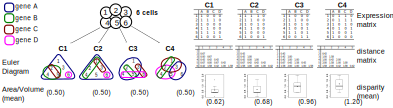
\includegraphics[width=0.95\textwidth]{./Images/measures_relations.png}
  \centering
  \caption{\textbf{Relation between area/volume of expression and disparity measures.} An embryo of six cells (top left) is shown expressing four different gene expression combinations (C1, C2, C3 and C4) of four genes (A, B, C and D). All combinations have a mean relative area/volume of 0.5. Each gene expression configuration is represented as an Euler diagram (representing the subset of the cells in which it is expressed in a color code shown at the top left) and as binary expression matrix (top right). The pairwise distance between the cells, calculated as 1-(pearson's correlation), is shown as a matrix. At the bottom right, a distribution plot of the pairwise distances of each combination and the mean disparity are shown below in parenthesis.
 }
  \label{fig:measures_relations}
\end{figure}
%%%%%%%%%%%%%%%%%%%%%%%%%%%%%%%%%%%%%%%%%%%%%%%%%%%%%%%%%%%%%%%%%%%%%%%%%%%%%%%%%%%%%


	\section{Data mining and handling}
	The work presented here is mainly based on the analysis of publicly available data contained in many databases, shortly introduced in the Review of the Literature section. In the next paragraphs I will describe how the data used in here was acquired and processed, for the details, see the corresponding study.

\subsection{In situ Hybridization data}

\subsubsection{\textit{D. melanogaster} (study I and III)}

\paragraph{Image acquisition and filtering}

Images were downloaded from the FlyExpress Database version 5.1 \citep{Kumar2011} on February 2013. Only genes with laterally oriented images for the six stages used in BDGP \citep{Tomancak2002} were considered.

Images were systematically retrieved and resized to 320 x 128 pixels (as in \citealp{Konikoff2012}) with ad-hoc Perl scripts. 
The gene expression pattern was obtained selecting one of three filtered images, obtained with an adaptive threshold based on the mean and variance of a grey-scale version of each image (see study I for details). Genes with ubiquitous expression in stages 1-3 and 4-6 were considered as entirely black images.

To correct for small variation in the shape of the embryos I adjusted each embryo to an stage ideal embryo shape, with an algorithm I made to morphometrically deform the real embryo contour of each image to the corresponding stage ideal shape.
Finally I applied a "smoothing filter" and eliminate isolated white/black pixels. 
I also manually filtered images from the literature or directly from BDGP of Transcription Factors or Growth Factor genes that did not have information in FlyExpress. 
For study I, the resulting dataset contained 1218 genes with expression information in the six stages used in BDGP. For study III, after updating the gene identifiers, repeated genes were removed, leaving a dataset of 1199 genes. \textbf{CHECK}

\paragraph{Anatomical terms}
In addition to the whole-mount in situ RNA-hybridization images, the BDGP database contains, for each gene, the list of the embryonic anatomical structures in which such gene is expressed \citep{Tomancak2007}. Each gene expression is described by one or several of those of anatomical terms by an expert. 
This information was retrieved from the BDGP downloads page (http://insitu.fruitfly.org/ insitu/html/ downloads.html/), which contains the annotations of almost 8,000 genes. We removed genes with "no staining" as anatomical term in any stage, leaving a total of 5762 genes.

\subsubsection{\textit{C. intestinalis} (study II)}

I downloaded the in situ hybridization data (ish.zip file) from the download section of the ANISEED database on 28th of December 2015. 
The expression data for the first three stages is at the cell level, while in the tailbud stages is at the tissues or specific regions of the embryo level. 
I extracted the information of the 32 cells, 64 cells, 112 cells, early tailbud, mid tailbud and late tailbud stages. Only expression data from experiments reported to have Wild type phenotype, "public" publication status, with in situ hybridization as experiment design and whose probe was assigned to a Kyoto Hoya (KH) \citep{Satou2008} gene model.
I excluded data from experiments whose image characterization was reported as "not sure" or too broadly as "part of whole embryo".

The number of genes analyzed is n=745 for the 32-cell stage, n=758 for the 64-cell stage, n=809 for the 112-cell stage, n=1082 for the early tailbud, 1092 for the mid tailbud and 887 for the late tailbud. 

\paragraph{Transcription factors and signalling genes}
I used the comprehensive list of TFs (http:// ghost.zool.kyoto-u.ac.jp/ TF\_KH.html) and SIGs (http:// ghost.zool.kyoto-u.ac.jp/ ST\_KH.html) deposited in the Ghost database (last access in July 2015).
 
This list is based mainly in \citet{Imai2004}, who determined the expression profiles of 389 transcription factors (TFs) and 118 signaling molecules (SIGs) genes from the egg to mid-tailbud embryos. TFs are categorized in nine gene families: basic helix-loop-helix (bHLH), homeodomain (HD), Fox, ETS, bZIP, nuclear receptor (NR), HMG, T-box transcription factors or as "other TFs" (mainly with diverse Zinc finger genes).
The SIGs genes consist of genes of receptor tyrosine kinase pathways including ligands such as FGFs and intracellular signalling molecules such as MAPK, Notch, Wnt, TGF$\beta$, Hedgehog and genes in the JAK/STAT pathways. 

\paragraph{3D embryo models}

I downloaded from the ANISEED database (from the biometry.zip folder; for more details see study II) files with a quantitative description of the geometry of individual blastomeres of the 32-cell, 64-cell and 112-cell stages. These files include the volume of each blastomere in percentage of the whole embryo \citep{Tassy2006}, used in the relative volume analysis.

Also, I downloaded 3D embryo models for these stages from the ANISEED database, available at a single-cell resolution. 
For the tailbud stages I used a 3D model of \textit{Ciona intestinalis} mid tailbud (stage 22) anatomy at a single cell resolution \citep{Nakamura2012}, downloaded as a file "3DVMTE\_THratio1.86.wrl" from http://chordate.bpni.bio .keio.ac.jp/3DVMTE/.
From this file, I manually extracted the information of different tissues into separate 3D files and processed them using diverse filters of the Meshlab software version v1.3.3\_64bit (Meshlab Visual Computing Lab ISTI-CNR; see study II for details).

\subsection{Transcriptomics and population genomic data}

\paragraph{modENCODE (study III and IV).}

Gene expression levels in reads per kilobase per million mapped reads (RPKM) units for 30 developmental stages were retrieved from \citet{Gelbart2013}, who analyzed RNA-seq throughput data from the modENCODE project \citep{Graveley2011}.

For using RNA-seq data to compare expression between samples, a normalization step was performed to adjust for varying sequencing depths and other potential technical effects across replicates (see study III)

\paragraph{DGRP (study III and IV).}

The population genomic data comes from 168 inbred lines of \textit{D. melanogaster} sequenced in the Freeze 1.0 of the Drosophila Genetic Reference Panel (DGRP) project \citep{Mackay2012}. The DGRP population was created collecting gravid females from a single population of Raleigh, North Carolina (USA), and following the full-sibling inbreeding approach during 20 generations to obtain full homozygous individuals. 
DGRP lines showing high values of residual heterozygosity (>9\%) that were observed to be associated with large polymorphic inversions \citep{Huang2014} were not included.

\paragraph{Testes and immune genes (study III).}
To discard the possibility that the adaptation patterns are due to an excess of male-biased genes, testes specific genes or immune-related genes, known of being under positive adaptation \citep{Civetta1995,Swanson2001,Artieri2009,Obbard2009}, genes related to these functions were removed (for details see Methods study III).

\paragraph{Maternal, maternal-zygotic and zygotic genes (study III).}
A list of maternal, semi-maternal and zygotic genes was obtained using data from \citet{Thomsen2010}, who performed microarray analyes of unfertilized eggs and the early zygote embryos (for details see Methods study III).

	\section{Estimating adaptation with DFE-alpha}
	
To estimate adaptation during \textit{D. melanogaster} embryogenesis, the DFE-alpha method and software were used (see section \ref{alpha}; \citealp{Eyre-Walker2009}), which infer adaptation combining polymorphism and divergence data.

The DFE-alpha software (DFE-alpha, \citealp{Eyre-Walker2009}; see below) requires that all sites to have been sampled in the same number of chromosomes. Therefore, the original DGRP dataset was reduced to from 168 to 128 isogenic lines by randomly sampling the polymorphisms at each site without replacement. Residual heterozygous sites and sites with no quality value were excluded from the analysis.
%
This software estimate several parameters (e.g., $\alpha$ and $\omega_{\alpha}$) from a set of genes as estimates based on single genes can be affected by the lack of segregating (divergent) sites. Therefore, in each analysis a group of genes was randomly sampled (bootstrap with replacement) (see studies III and IV). 
As neutral reference the positions 8-30 of short introns ($\leq$ 65 bp) were used (as in \citealp{Heyn2014}). For validation, 4-fold degenerate sites were also used.

The release 5 of the Berkeley Drosophila Genome Project was used as the reference genome (http://www.fruitfly.org/sequence/release5genomic.shtml/). The divergence statistics were estimated from a multiple genomic alignment between DGRP lines and \textit{D. yakuba} BDGP 5 coordinates (from http://popdrowser.uab.cat; \citealp{Ramia2012}).
The number of sites and substitutions and the folded site frequency spectrum (SFS) were computed using an ad hoc Perl script.

Ortholog genes between \textit{D. yakuba} and \textit{D. melanogaster} were obtained from FlyBase (http://flybase.org/). \textit{D. yakuba} was used as outgroup species as, due to the time since their divergence, there is less chance of ancestral polymorphism contributing to divergence, diminishing the effect of low divergence affecting the estimates of adaptive evolution \citep{Keightley2012}.

	\section{Transcriptome age and genomic determinants}
	\subsection{Transcriptome age}

\subsubsection{Gene phylogenetic age}
A phylogenetic age to each gene was assigned using the phylostratigraphic maps of \textit{D. melanogaster} (from \citealp{Drost2014}). The age assigned to each gene is based on the phylogenetic level at which ortholog genes are found. 
Therefore, each gene is assigned to a discrete age category, or phylostratum (PS), corresponding to hierarchically ordered phylogenetic nodes along the tree of life database \citep{Drost2015}. 
	\nomenclature{PS}{Phylostratum}

I downloaded the PS dataset on May 2015 (available from http://dx.doi.org/ 10.6084/ m9.figshare.1244948/). For study III, the number of analysable genes for the spatio-temporal and anatomical term analyses were 555 and 2722 genes, respectively (genes with PS values and analysable with the DFE-alpha method, see above).


\subsubsection{Region phylogenetic age} 

The Transcriptome Age Index (TAI) is defined as the weighted arithmetic mean of phylostrata, using gene expression intensities as weights \citep{Domazet-Loso2010}.
	\nomenclature{TAI}{Transcriptome Age Index}

In here, I calculated the TAI for each region and territory of the embryo in a developmental stage, using the relative area of expression of a gene in a region or territory as weights instead of the expression intensity.
Therefore, for each region and territory $j$, the TAI was calculated as:
%
$$ TAI_{j} = \frac{ \sum_{i=1}^{n} ps_{i}A_{ij} }{ \sum_{i=1}^{n} A_{ij} }$$
%
where $ps_{i}$ denotes the PS of gene $i$ , $A_{ij}$ is the relative area of gene $i$ in the region or territory $j$, and $n$ the number of genes expressed in such region or territory. A relatively low value of $TAI_{j}$ represents a high mean evolutionary age of the transcriptome in the region or territory j, and conversely. The TAI was calculated using the myTAI R package \citep{Drost2014}.

%\subsubsection{Genomic determinants}

The following genomic features, called in here "genomic determinants" were obtained using coding exons and short introns annotations for \textit{D. melanogaster}, obtained from FlyBase release 5.50. 

\textbf{Intron length.} Average distance, in base pairs, between the exons of a gene.

\textbf{Intergenic distance.} Average number of base pairs between two adjacent genes.

\textbf{Gene size.} Length of the coding region of a gene.

\textbf{Messenger complexity.} Number of transcripts divided by the total number of exons.

\textbf{Number of transcripts and exons.} Number of different transcripts and exons of a gene, respectively.

\textbf{Codon bias.} Measured as the Frequency of optimal codons (Fop). Was estimated using CodonW (\citealp{Peden1999}; http://codonw.sourceforge.net/).
	\nomenclature{Fop}{Frequency of optimal codons (a measure of codon bias)}
This index is estimated as the ratio of optimal codons to synonymous codons. Its values range between 0, where no optimal codons are used, and 1, where only optimal codons are used.

\textbf{Expression bias.} Proportion of development stages in which a gene is expressed. Based on \citep{Yanai2005} and \citep{Larracuente2008}, we estimated the expression bias, $\tau$ as:
%
$$ \tau = \frac{ \sum_{j=1}^{n} 1- \log S_{j} / \log S_{max} }  { n-1 } $$
%
where $S$ is the logarithm of the RPKM and $n$ is the number of developmental stages. $\tau$ ranges from 0 to 1, with values close to 0 indicating broadly expressed genes and values close to 1 indicating genes with highly biased expression.

\textbf{Expression level.} Estimated as the logarithm of the maximum expression in RPKM units.

\textbf{Recombination levels.} Recombination rates estimates at 100 kb non-overlapping windows, crossing-over events (from \citealp{Comeron2012}).

%%Testes and immune genes
%%In order to discard that the adaptation patterns found are due to an excess of male-biased genes, testes specific genes or immune-related genes, that are known of being under positive adaptation[31,50–52], we removed genes related to this functions [72]. For that, we downloaded the Gene Ontology (GO) terms for our gene set through the R package biomaRt [73] using the D. melanogaster ENSEMBL database. When a gene was associated to any of those terms, it was removed for performing the analysis.


%\input{./Parts/Methods}
\clearpage

%%%% -----------------------------------------------------------------
%%%% -----------------------------------------------------------------
	
\chapter{Results and Discussion}

%\section{Complexity and compartmentalization in \textit{Drosophila}}
%	\subsection{Area of expression decreases non-linearly}

The mean area of expression decreases in a non-linear way (an inverted saturation curve), with the major decrease occurring at very early development, from maternal to early gastrula stage (Fig. \ref{fig:Art-I-Area}).

This pattern of decrease is observed both in maternal genes (genes that are expressed from stage (1) and in zygotic genes (genes that start to be expressed later).
This highlight that a great proportion of the genes have already a restricted spatial pattern at early gastrulation, therefore the embryo is relatively well compartmentalized at this stage.

%Practically half of the genes in our set follow this decrease pattern: 46 of the genes (565 of 1218 genes) were characterized as having a non-linear decrease in their relative area (Appendix. S1). Our results are consistent with the hypothesis that the Drosophila embryo becomes compartmentalized in a progressively more fine-grained manner over developmental time. This is, most genes start being expressed in broad areas of the embryo and over time their expression becomes progressively restricted into smaller and smaller spatial domains.

\begin{figure}[h]
  \includegraphics[width=0.4\textwidth]{./Images/Art-I/area.png}
  \centering
  \caption{Distribution plot of the relative area of expression for all genes in each stage. Diamonds represent the mean, boxes the IQR. Whiskers 10 and 90 percentiles. Dashed line represents the max values and dotted line the min values (mean of the last and first decile, respectively). Stages on the x-axis, vertical dashed line represents gastrulation entry.}
  \label{fig:Art-I-Area}
\end{figure}

%%%%%%%%%%%%%%%%%%%%%%%%%%%%%%%%%%%%%%%%%%%%%%%%%%%%%%%%%%%%%%%%%%%%%%%%%%%%%%%%%%%%% 

\subsection{TFs and GFs compartmentalize earlier}
The transcription factors (TFs;GO:0003700) and growth factor genes (GFs;GO:0008083) showed significantly smaller relative area of expression that the other genes in the blastoderm stage (Fig. \ref{fig:Art-I-TF-GF_area}).
	\nomenclature{GF}{Growth Factor}
	\nomenclature{KW}{Kruskal-Wallis test}
	
The TFs are expressed in significantly smaller areas than the rest of the genes in subsequent stages and the GFs are expressed in smaller areas at the blastoderm stage (stage 4-6) and the extended germ band stages (stage 9-10 and 11-12) (KW pvalue $<$ 0.05, Fig. \ref{fig:Art-I-TF-GF_area}).

 The fact that these genes have lower relative area (i.e., are more compartmentalized) than the rest of the genes, especially in the stage before entering gastrulation, is consistent with the leading role of these genes in driving pattern formation and the resulting compartmentalization of the embryo.
 
\begin{figure}[h]
  \includegraphics[width=0.8\textwidth]{./Images/Art-I/TF-GF_area.png}
  \centering
  \caption{Comparison between the relative area of expression of the transcription factors (white boxes) with the rest of the genes (gray boxes). On the right, same comparison for the growth factors (white boxes) and the rest of the genes (gray boxes). Stars represent significant values of p-values from Kruskal-Wallis test (*$<$0.05, **$<$0.01,***$<$0.001). Number of genes indicated below each box. }
  \label{fig:Art-I-TF-GF_area}
\end{figure}

%%%%%%%%%%%%%%%%%%%%%%%%%%%%%%%%%%%%%%%%%%%%%%%%%%%%%%%%%%%%%%%%%%%%%%%%%%%%%%%%%%%%% 
\subsection{Spatial disparity}

The disparity measure informs about how different genetically are the different regions of the embryo in different stages. This is complementary to the relative area of expression, as it could be that between two stages the relative area of expression decreases but not the disparity if the genes are expressed in the same part of the embryo.
Fig. \ref{fig:Art-I-disparity} shows that the disparity increases non-linearly following again a saturation curve, with the major change in the early stages.
In the blastoderm stage the disparity of the regions based only on the TFs is much greater than the one based on all the genes ((KW pvalue $<0.001$; Fig. \ref{fig:Art-I-disparity}) indicating that these genes account for a large portion of the diversity of gene expression patterns.

\begin{figure}[h]
  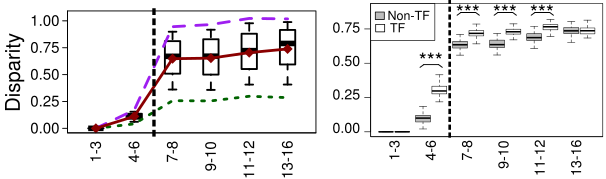
\includegraphics[width=0.8\textwidth]{./Images/Art-I/disparity.png}
  \centering
  \caption{Comparison between the relative area of expression of the transcription factors (white boxes) with the rest of the genes (gray boxes). On the right, same comparison for the growth factors (white boxes) and the rest of the genes (gray boxes). Stars represent significant values of p-values from Kruskal-Wallis test (*$<$0.05, **$<$0.01,***$<$0.001). Number of genes indicated below each box. }
  \label{fig:Art-I-disparity}
\end{figure}


%	\clearpage
%\section{Complexity and compartmentalization in \textit{Ciona}}
%	\subsection{Major increase in compartmentalization and disparity after gastrulation}
%objective
With \textit{Ciona}, I measured compartmentalization combining gene expression data at the individual cell-level (until gastrula) or tissue level (tailbud stages) with various 3D embryo models.
Therefore, in here I will refer to relative volume of expression (instead of area as previously)
%results
Globally, the volume of expression decreases mostly after gastrulation (between the 112-cell and the early tailbud stage).
However less dramatic, I found significant differences between the 32-cell and 64-cell stages, and between the 64-cell and 112-cell stages.

As expected, the major increase in disparity happens also occurs between the 112-cell and the early tailbud stage (II, Fig. 4).
I also found a significant increase in disparity in the 64 to 112-cell stages and early to mid-tailbud stages transitions.
Importantly, I found no significant differences between the relative volume of expression of the early and mid-tailbud (II, Fig. 3A), but I found a significant difference between their disparity.

%discussion

This means that, on average, genes are expressed in a similar number of tissues in these stages, but in the mid tailbud the combination of genes expressed in these tissues are more different between each other. This shows that the disparity measure is complementary to the relative volume measure to describe the compartmentalization of the embryo.

In contrast to what I found in \textit{Drosophila}, the major change in compartmentalization in \textit{Ciona} occurs clearly after gastrulation.
In \textit{Ciona}, early embryonic patterning is based on maternal determinants and signalling events mostly between neighbouring cells \citep{Lemaire2009}, which act in a combinatorial way \citep{Hudson2007} to establish a unique TF combination in more than half of the blastomere pairs before gastrulation \citep{Imai2006} determining most of their fates.
Thus, even when in \textit{Ciona} most of the cell fates are already determined (by the specific combination of a fraction of TFs) and the embryo can be said to be already highly compartmentalized, this is not evident at the global level of gene expression, which I am measuring here.
This `delay' could be explained by the relatively slower process of signal transduction (as in \textit{Ciona}) compared to the gap gene network (in \textit{Drosophila}).

%%%%%%%%%%%%%%%%%%%%%%%%%%%%%%%%%%%%%%%%%%%%%%%%%%%%%%%%%%%%%%%%%%%%%%%%%%%%%%%%%%%%% 
\subsection{The leading role of TFs and SIGs}
%objective
I then tested if in \textit{Ciona} the TFs and signalling molecules (SIGs) also showed an early compartmentalization, expected from their allegedly leading role in early pattern formation.
	\nomenclature{SIGs}{Signaling molecules}
	\nomenclature{RTK}{receptor tyrosine kinase}
SIGs consist of genes of receptor tyrosine kinase (RTK) pathways such as FGFs and intracellular signalling molecules such as MAPK, Notch, Wnt, TGF$\beta$, Hedgehog and genes in the JAK/STAT pathways (based on \citealp{Imai2004}) 

%results 1
As expected, TFs volume of expression decreased faster than non-TFs. The TFs showed lower volume of expression in the 64-cell and 112-cell stages (II, Fig. 3B). The results are similar for maternal and zygotic genes (maternal/zygotic classification based on \citealp{Matsuoka2013}; II,Fig. S1).
I then compared TF families (categories based on \citealp{Imai2004}) and found that six TF families showed lower relative volume in the early gastrula (BZIP, T-box, bHLH, HMG, Nuclear Receptor, and `Other-TFs') but only T-box genes showed a lower relative volume from the 32-cell stage until gastrula (II,Fig. S2). 

%discussion 1
The results obtained for the T-box gene family (conserved in metazoan and several non-metazoan lineages \citep{Sebe-Pedros2013}) are consistent with the known important role these genes have in diverse metazoan species early cell fate specification (reviewed in: \citealp{Papaioannou2014,Showell2004}.
Examples of T-box genes in \textit{Ciona} are Tbx6 and \textit{brachyury}, crucial for muscle tissue formation \citep{Mitani1999,Nishida2005} and for notochord specification \citep{Yasuo1998}, respectively.
 
%results 2
SIGs showed significant lower relative volume of expression than the rest of the genes in the 32-cell, 64-cell, and 112-cell stages (II, Fig. 3B).
Specifically, in the 64-cell stage RTK-MAPK, Wnt and TGF$\beta$ families showed significant higher disparity in the 64 cells stage, suggesting a predominant role of these pathways in the patterning of the embryo at this stage. 
%discussion2
This is consistent with known short range induction events by nodal and various FGFs, which are part of the TGF$\beta$ and RTK-MAPK signalling pathways, respectively \citep{Lemaire2008}.
%general discussion? (X)


%%%%%%%%%%%%%%%%%%%%%%%%%%%%%%%%%%%%%%%%%%%%%%%%%%%%%%%%%%%%%%%%%%%%%%%%%%%%%%%%%%%%% 
\subsection{3D roughness increases non-linearly}
%objective
In here I used the Dirichlet Normal Energy (DNE; \citealp{Winchester2016}) as a measure of complexity that considers the overall curvature of the 3D surface of a gene expression pattern.
Importantly, DNE can also be analysed at different spatial scales. 
	\nomenclature{DNE}{Dirichlet Normal Energy}
Therefore, DNE would be the 3D equivalent of the roughness measure I used for \textit{Drosophila}.

%results
DNE values increase throughout development (II, Fig. 5), again with the major change between the 112-cell and the early tailbud. 

The max (mean of the last decile) values increase substantially already between the 64 and 112 cells stages (with 1000 and 10000 polygonal faces), while the min values (mean of the first decile) remain practically constant during development, showing that the most complex patterns in each stage get increase their DNE value but there is always a proportion of very simple expression pattern.
Also, I found that at low spatial scales (1000 and 10000 polygons per mesh; II, Fig. 5) I found that the mean DNE of the late tailbud is higher than at the mid tailbud (one-way ANOVA pvals < 0.05).
	\nomenclature{ANOVA}{Analysis of Variance}

%discussion
In summary, this results show that the complexity of distribution in 3D space of cells/tissues expressing a gene (measured with DNE) increases through development, as even when the increase was more pronounced just after gastrulation, significant changes were found before and after this.

%%%%%%%%%%%%%%%%%%%%%%%%%%%%%%%%%%%%%%%%%%%%%%%%%%%%%%%%%%%%%%%%%%%%%%%%%%%%%%%%%%%%% 
\subsection{Synexpression territories in \textit{Ciona}}
%objective
Because in the tailbud stages the information is based on tissues and not on individual cells as the early stages, I analysed the synexpression territories (STs) of these stages separately by means of a hierarchical clustering (II, Methods). As in Drosophila, how the different STs cluster with each other is informative of the degree of differentiation between stages. If STs cluster with other STs in the same stage, it would mean that the majority of genes change their expression in a similar way over time independently of where they are. If STs cluster with other STs in the same part of the
embryo in successive stages, it would mean that this part of the embryo has expression dynamics independent from other parts of the embryo, which would be expected in already differentiated cells/tissues.

%results
Early stages STs cluster by stage. Thus, even if at the first three stages a high proportion of blastomeres express a nearly unique combination of transcriptional factors \citep{Imai2006}, the bulk change in gene expression is common to all blastomeres. Within each early stage, STs coincides very well with the know fate map (II, Fig 6A; II, Fig. S8), with some exceptions That I describe in the next subsection.

In contrast, in tailbud stages practically all STs cluster by tissue/cell type, which indicates that the in early tailbud, most tissues are already quite differentiated.
This is largely consistent with the bulk of other studies analyzing these stages at the level of individual or small sets of genes \citep{Corbo1997,DiGregorio1999}.

%discussion 2
The early stages analysis is similar to one made by \citet{Imai2006}, who used the expression profile of 53 zygotically TFs in single cells in the 16, 32, 64, and 112-cell stages, to perform a hierarchical clustering (for each stage separately). My analysis is different in two aspects: I performed the clustering using the blastomeres of different stages and my analysis is not restricted to TFs. As I said previously, using various stages is informative of the overall differentiation process and can be used to discern between differentiation scenarios, as the differences between early and tailbud stages I found here.

\begin{figure}[h]
  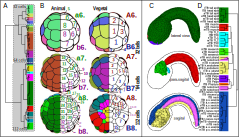
\includegraphics[width=\textwidth]{./Images/Art-II/territories.png}
  \centering
  \caption{Ciona synexpression territories. 
  (A) Dendrogram produced by hierarchical clustering of cells in 32-cell, 64-cell and 112-cell stages. Dashed boxes show that STs cluster by stage. Coloured boxes show the cut-off to produce 24 STs.
  (B) Names of cells (Conklin nomenclature; \citealp{Conklin1905}) indicated with a prefix shown at right. STs in the 32 cells, 64 cells and 112 cells stages (top, middle and bottom, respectively). Colour refers to which ST of the dendrogram (in A) each cell is part of. Animal view based on \citet{Nicol1988} and vegetal view based on \citet{Cole2004a}. The cell marked with a star (*) is the A7.6 cell, that in this analysis represents their descendant cells (A8.11 and A8.12).
  C) Dendrogram produced by hierarchical clustering of tissues in early, mid and late tailbud stages. The coloured boxes show the cutoff to produce 10 STs. (D) STs in the tailbud stages shown in a lateral, para-sagital and sagital views of a mid tailbud 3D embryo model (from \citealp{Nakamura2012}). Colour refers to which ST of the dendrogram (in C) each tissue is part of.
}
  \label{fig:Art-II-territories}
\end{figure}

%%%%%%%%%%%%%%%%%%%%%%%%%%%%%%%%%%%%%%%%%%%%%%%%%%%%%%%%%%%%%%%%%%%%%%%%%%%%%%%%%%%%% 
\subsection{Discrepancies between fate map and STs}

I found a few cases in which cells with the same fate where contained in different STs. This would be the case of: 1) cells whose fate is disproportionally affected or determined by a small number of genes (as this analysis reflect quantitative differences at the level of hundreds of expressed genes
but can not distinguish between the relative importance of each gene) or 2) cells that although having a restricted fate at a certain stage their differentiation is not complete (at the level of gene expression).

An example of the latter is a ST in the 112-cell stage (in magenta; Fig. X) that contains   precursors of the notochord (A8.5, A8.6, A8.13, and A8.14, B8.6) and mesenchyme (B8.5) \citep{Tokuoka2004}.
The latter come from a secondary notochord/mesenchyme bipotential cell (B7.3). It has been reported that the expression of Twist-like 1, necessary for mesenchyme differentiation, starts at this stage \citep{Imai2003}.
This evidence, together with the inclusion of the mesenchyme cell in this otherwise exclusively notochord territory (primary and secondary), seems to indicate that the differentiation of cell pair B8.5 as mesenchyme is still incomplete at this stage.

\subsection{Gene expression dynamics in cell-lineages}

I analysed the gene expression similarity between lineage-related cells (i.e., between daughters cells and between mother/descendants cells) in the early stages (II, Fig. 8).
In general, cells are more closely genetically to their sister cells than to their mother/descendants, which is reflected in the clustering of STs by stages discussed before.
I found also that at the 64-cell stage, cells that show more genes expressed differently than
their ancestors are neural fated cells, which might be related with the fact the unrestricted state of these cells at this stage (i.e., their descendants will give rise to different cell fates).
%	\clearpage

%\section{Compartmentalization and complexity measures}
%	\input{./Parts/Results_Art_.tex}
%	\clearpage

\section{Comparative study between \textit{Drosophila} and \textit{Ciona} (I and II)}
	\subsection{Compartmentalization}
%objective
I estimated the degree of compartmentalization calculating the relative area or volume of expression of genes during development.
My intention here was not to focus on individual genes, but to get a global overview of the embryo compartmentalization and differentiation processes based on expression data of thousands of genes, i.e., using a statistical approach.

One would expect, and it has been implicitly assumed \citep{Carroll2001} \citep{Davidson2001} that the compartmentalization of the embryo (as I measure it here) increases during development.
However, the specific temporal dynamics of this increase in any species is not known. Neither is clear if the dynamics should be similar for different species, or for different groups of genes.
As the development of \textit{Ciona} and \textit{Drosophila} are very different and it would be impossible to compare them stage-by-stage, I focused here in three major developmental periods: pre-gastrula, gastrula, and post-gastrula stages. These periods are easily recognizable in both species facilitating the comparative analysis.

%results
I found that in both species, the relative area or volume decreased in a non-linear way (see Figs X). 
However, the timing of the major decrease was different.
In \textit{Drosophila} the major decrease occurred at very early development, from maternal to early gastrula stage (Fig. \ref{fig:Art-I-3measures}).
Practically half of the genes in follows this decrease pattern: 46\% of the genes were characterized as having a non-linear decrease in their relative area.
In contrast, in \textit{Ciona} the volume of expression decreases mostly after gastrulation (between the 112-cell and the early tailbud stage).
However less dramatic, I found significant differences between the 32-cell and 64-cell stages, and between the 64-cell and 112-cell stages.

\begin{figure}[h]
  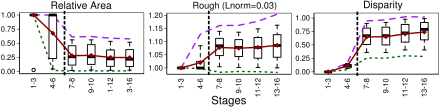
\includegraphics[width=\textwidth]{./Images/Art-I/3_measures.png}
  \centering
  \caption{Distribution plot of the relative area of expression (left), roughness (center) and disparity (right) for all genes in each stage. Diamonds represent the mean, boxes the IQR. Whiskers 10 and 90 percentiles. Dashed line represents the max values and dotted line the min values (mean of the last and first decile, respectively). Stages on the x-axis, vertical dashed line represents gastrulation entry.}
  \label{fig:Art-I-3measures}
\end{figure}

% discussion
The difference in the timing of the major change on compartmentalization between species must relate to differences in their specific development.

The earlier compartmentalization of \textit{Drosophila} is most probably due to its derived early development, namely, the syncytial blastoderm. 
During the blastoderm stage, approximately 4,000 cell nuclei can `communicate' with each other only by TFs \citep{Jaeger2011}. The direct cross regulation of gene expression facilitates a rapid and highly dynamic process which seems to be responsible for the early spatial restriction of a great proportion of developmental genes.

In contrast,  \textit{Ciona}'s early embryonic patterning is based on maternal determinants and signalling events mostly between neighbouring cells \citep{Lemaire2009}, which act in a combinatorial way \citep{Hudson2007} to establish a unique TF combination in more than half of the blastomere pairs before gastrulation \citep{Imai2006} determining most of their fates.
Thus, even when in \textit{Ciona} most of the cell fates are already determined (by the specific combination of a fraction of TFs) and the embryo can be said to be already highly compartmentalized, this is not evident at the global level of gene expression, which I am measuring here.


Therefore, the `delay' of compartmentalization observed in \textit{Ciona} could be explained by the relatively slower process of signal transduction (as in \textit{Ciona}) compared to the gap gene network (in \textit{Drosophila}).

%%%%%%%%%%%%%%%%%%%%%%%%%%%%%%%%%%%%%%%%%%%%%%%%%%%%%%%%%%%%%%%%%%%%%%%%%%%%%%%%%%%%%
\subsection{Disparity}
%objective
As the relative area (or volume) of expression informs on how genes are expressed in progressively smaller regions in the embryo, the disparity can inform about how different regions of the embryo express increasingly different combinations of genes.

Therefore, both measures reflect slightly different aspects of complexity that are independent from each other. A decrease in the volume of expression of genes does not necessarily imply an increase in spatial disparity: genes could decrease their volume of expression but end up restricted to the same parts of the embryo. 
If the majority of genes would be expressed ubiquitously (this is large volume), however, then the mean disparity between its regions would be necessarily low. 

%results
My results show that in each species, the global disparity pattern is similar to the relative area or volume patterns.
Therefore, in Drosophila the disparity increases mostly in the transition from the maternal to early gastrula and in Ciona this major change occurs after gastrulation.

FIGURA CIONA 3 MEDIDAS

% discussion
It is important to notice that these measures should not necessarily correlate, as it could be that between two stages the relative area of expression decreases but not the disparity if the genes are expressed in the same part of the embryo or vice-versa.

In \textit{Ciona} I found an example of such case, when there is no perfect correspondence between the relative volume and the disparity of expression: disparity increased significantly between early to mid-tailbud stages but no significant differences between the relative volume of expression of these stages were found (II, Fig. 3A).

This means that, on average, genes are expressed in a similar number of tissues in these stages, but in the mid tailbud the combination of genes expressed in these tissues are more different between each other. This shows that the disparity measure is complementary to the relative volume measure to describe the compartmentalization of the embryo.


%%%%%%%%%%%%%%%%%%%%%%%%%%%%%%%%%%%%%%%%%%%%%%%%%%%%%%%%%%%%%%%%%%%%%%%%%%%%%%%%%%%%% 
\subsection{2D and 3D roughness analyses}




%%%%%%%%%%%%%%%%%%%%%%%%%%%%%%%%%%%%%%%%%%%%%%%%%%%%%%%%%%%%%%%%%%%%%%%%%%%%%%%%%%%%% 
\subsection{Synexpression territories}

%	\clearpage

\section{Main spatio-temporal profiles of gene expression in \textit{Drosophila} (I)}
	%objective
With a time series cluster analysis \citep{Ernst2006} of the relative area of expression, I found the eight main spatio-temporal profiles of gene expression in the embryonic development of \textit{Drosophila} (I, Fig. 5).
%results
As expected, the most common profile (n=297 genes) follows the global profile of non-linear decrease in the first stages (I, Fig 5).

Among the rest of profiles, I found both linear increase and decrease profiles and a `hill-like' profile (initial increase and further decrease with the higher values at stage 7-8)
%
The linear decrease profile (n=167 genes) was enriched with `mitotic cell cycle' (GO:0000278), `RNA processing' (GO:0006396) and `chromatin modification' (GO:0016568) GOterm genes, highlighting biological processes that first are present in the whole embryo and become more and more restricted in space as development proceeds.
%discussion
The `mitotic cell cycle' term, for example, most likely relates to the fast mitotic cycles in the earliest embryo. During stage 1-3 nine fast and synchronic mitotic divisions take place in the entire embryo, then in stage 4-6 mitotic divisions 10-13 occur more slowly, almost synchronically. The 14th cycle, zygotically controlled, is long and of different durations in the embryo.

With a temporal co-expression cluster analysis using microarray data through the life cycle of \textit{D. melanogaster}, \citet{Arbeitman2002} found that most cell cycle genes were expressed at high levels during the first 12h, but only a few are expressed at high level thereafter.
My analysis is consistent with this, as I found that the profile of linear decrease (I, Fig. 5A) is enriched with such genes. In this sense, this study is complementary to Arbeitman et al., and adds the spatial dimension to their temporal expression profiles.

%	\clearpage

\section{Discrepancies between fate map and STs (II)}
	
I found a few cases in \textit{Ciona} in which cells with the same fate where contained in different STs. As explained in section X, it would be expected that a fate map would largely coincide with a gene expression map. This analysis could not be made in \textit{Drosophila} as the gene expression data is not a the single level resolution.

A lack of correspondence, as it was found in here, could be due to: 1) cells whose fate is disproportionally affected or determined by a small number of genes (as this analysis reflect quantitative differences at the level of hundreds of expressed genes but can not distinguish between the relative importance of each gene) or 2) cells that although having a restricted fate at a certain stage their differentiation is not complete (at the level of gene expression).
%
An example of the latter is a ST in the 112-cell stage (in magenta; \ref{fig:Art-II-territories} B; II, Fig. S8) that contains precursors of the notochord (A8.5, A8.6, A8.13, and A8.14, B8.6) and mesenchyme (B8.5) \citep{Tokuoka2004}.
The latter come from a secondary notochord/mesenchyme bipotential cell (B7.3). It has been reported that the expression of Twist-like 1, necessary for mesenchyme differentiation, starts at this stage \citep{Imai2003}.
This evidence, together with the inclusion of the mesenchyme cell in this otherwise exclusively notochord territory (primary and secondary), seems to indicate that the differentiation of cell pair B8.5 as mesenchyme is still incomplete at this stage.

\subsubsection{Gene expression dynamics in cell-lineages}

During \textit{Ciona} early embryogenesis, I analysed the gene expression similarity between lineage-related cells i.e., between daughters cells and between mother/descendants cells (II, Fig. 8).
In general, cells are more closely genetically to their sister cells than to their mother/descendants, which is also reflected in the clustering of STs by stages discussed before.
I also found that at the 64-cell stage, cells that show more genes expressed differently than their ancestors are neural fated cells. This could be related with the change from unrestricted state of these cells at this stage (i.e., their descendants will give rise to different cell fates) to a restricted state in the next stage (112-cell stage) \citep{Imai2006}.
Therefore, it could be hypothesized that when a cell changes from a unrestricted to a restricted cell fate state, a major change in gene expression should be evident when following gene expression dynamics of its cell-lineage.  
%	\clearpage

\section{Adaptation in \textit{Drosophila} embryogenesis (III and IV)}
	%% objective

I combined the Synexpression Territories (STs) approach with genome-wide coding-region polymorphism data (from the DGRP database) and the coding-region divergence between \textit{D. yakuba} and \textit{D. melanogaster} in order to estimate the  proportion of adaptive non-synonymous substitutions ($\omega_{\alpha}$) in the genes expressed in each ST (n=589 genes; III, Methods).
	\nomenclature{$\omega_{\alpha}$}{Proportion of adaptive non-synonymous substitutions}

Using this approach, I could chart a spatial map of natural selection acting on \textit{Drosophila}'s embryo anatomy.
I complemented this with a analysis using available annotation of gene expression (n=2,835 genes) using a controlled vocabulary of anatomical structures from the BDGP database \citep{Tomancak2007}.

%% results %%%%%%%%%%%%%%%%%%%%%%%%%%%%%%%%%%
The results showed a few STs with significant higher or lower $\omega_{\alpha}$ (permutation test; III, Methods)

%% high OmegaA
\subsection{STs or anatomical terms with high $\omega_{\alpha}$}
STs 13 and 32 (ST number comes from the hierarchical clustering algorithm), which showed a higher $\omega_{\alpha}$, seem to correspond to the forming foregut and hindgut (stage 11-12) and to the CNS (stage 13-16) respectively.
To explore if ST 32 high $\omega_{\alpha}$ was indeed related to the CNS, I separated the genes CNS or not-CNS related.
I found that both groups showed a high $\omega_{\alpha}$, which suggests that in addition to the CNS, another structure in the anterior region would be under positive selection.
 Using the anatomical terms approach, no anatomical terms related to the CNS were found to have high $\omega_{\alpha}$ with the initial criteria.
I therefore applied a more stringent criterion to consider genes as part of an anatomical term (before a gene could have a maximum of seven anatomical terms associated instead of a more stringent number of three) and found that `Embryonic brain' showed high $\omega_{\alpha}$ (permutation test, p = 0.046).
Also, with the anatomical terms approach, I found that genes associated with `Gonads', in the last stage, clearly showed evidence of adaptive evolution (III, Figure 2).

The evidence of adaptation in in agreement with previously reported high rates of adaptive substitution in the testes \citep{Akashi1994,Civetta1995,Nuzhdin2004,Proschel2006}

%% low omegaA
\subsection{STs or anatomical terms with low $\omega_{\alpha}$}
STs 20 and 29 with showed low $\omega_{\alpha}$, seem to correspond to the forming midgut (stage 11-12) and to the forming larval digestive system (stage 13-16) respectively.
Similar results are found when using the anatomical term approach, as low $\omega_{\alpha}$ was found in many anatomical terms related to the digestive system in the last stage: `Embryonic midgut', `Embryonic salivary gland', `Embryonic hindgut', `Embryonic proventriculus'. 
Also, combining three related anatomical terms, `Embryonic foregut', `Embryonic epipharynx' and `Embryonic hypopharynx', that separately did not have enough genes to be considered in the analysis, showed low $\omega_{\alpha}$. 

The lack of adaptive change in the forming digestive system might reflect their relative enrichment in metabolic genes \citep{Marianes2013}. The coding regions of metabolic genes have been found to be more conserved than non-metabolic genes \citep{Peregrin-Alvarez2009}.


%%%%%%%%%%%%%%%%%%%%%%%%%%%%%%%%%%%%%%%%%%%%%%%%%%%%%%%%
\begin{figure}[h]
  \includegraphics[width=0.8\textwidth]{./Images/Art-III/OmegaA_territories.png}
  \centering
  \caption{\textbf{$\omega_{\alpha}$ on embryonic territories over space and time.}
   Territories drawn in red in the central column mark significantly high $\omega_{\alpha}$ while those in blue mark significantly low $\omega_{\alpha}$ in space in each of the 6 developmental stages (rows). Other columns depict $\alpha$, the proportion of base substitutions fixed by natural selection, and $\omega$, the rate non-synonymous substitutions relative to the mutation rate. 
  Territories in dark gray are territories without enough specific genes to be analyzed. The statistical was calculated by a permutation test using all the genes analyzed (see Material and methods). Territory 13 in stage 9-10 ($\omega_{\alpha}$: 0.059, p = 0.045). Territory 20 from stage 11-12 ($\omega_{\alpha}$: 0.022, p = 0.048; $\alpha$: 0.259, p = 0.028). Territory 24 from stage 11-10 ($\omega_{\alpha}$: 0.070, p = 0.061). Territory 29 from stage 13-16 ($\omega_{\alpha}$: 0.037, p = 0.047; $\omega$: 0.074, p < 0.001). Territory 32 from stage 13-16 ($\omega_{\alpha}$: 0.068, p = 0.044; $\alpha$: 0.71, p = 0.04).
  }
  \label{fig:Art-III-OmegaA_territories}
\end{figure}
%%%%%%%%%%%%%%%%%%%%%%%%%%%%%%%%%%%%%%%%%%%%%%%%%%%%%%%%


\subsection{Transcriptome age index}

We also measured the phylogenetic age \citep{Drost2015} of the genes expressed in each territory, that is, the phylogenetic level at which orthologs for a gene are found (e.g., if a gene has orthologs among eukaryota the phylogenetic age is older than if a gene has orthologs only among Drosophilids). 

The territories where we found low rates of coding-region adaptive evolution express genes that are, on average, older than the genes expressed elsewhere (Figure 3). Similar results are found for anatomical structures (Figure S2).

We also found that in the latest stages the mean phylogenetic age of the genes expressed in the endoderm is lower than that of the genes expressed in other germ-layers, specially compared to the ectoderm (Figure 3). Similar results were found by \citep{Domazet-Loso2007} but without comparing stages.

Our analysis also shows that the embryo regions with high rates of adaptive substitution have low codon bias \citep{Sharp1991,Betancourt2002,Haerty2007} and, as previously reported \citep{Plotkin2011}, regions with high codon bias have high levels of gene expression (measured by RNA as reported in modENCODE \citep{Graveley2011} and averaged per region; see Materials and methods) (see Figure 4).

This latter correlation, however, was larger for regions with low $\omega_{\alpha}$ than for regions with high $\omega_{\alpha}$ (Figure 5A). Figure 5 shows that genes in regions with high $\omega_{\alpha}$ exhibit low codon bias relative to gene expression levels. The same relationship between $\omega_{\alpha}$ and codon bias is found in territory 32, the territory showing the stronger evidence of adaptive substitution (Figure 5).

%	\clearpage
\section{Adaptation trough \textit{Drosophila} life cycle (IV)}
	%% objective
%Using the modENCODE developmental data \citep{Graveley2011}, with expression data for 30 stages of the whole life cycle of \textit{D. melanogaster} (12 embryonic at 2-h intervals for 24 h, 6 larval, 6 pupal and 3 sexed adult stages at 1, 5 and 30 days after eclosion), $\omega_{\alpha}$ and other evolutionary rates for the genes expressed in each stage (for details see: IV, methods) were estimated.
%For each stage, $\omega_{\alpha}$, $\omega$, $\omega_{d}$ and $\alpha$ (Fig. \ref{fig:Art-IV-OmegaA_lifecycle}) were estimated with the differentially expressed genes (genes with expression different from zero and excluding those expressed in all stages).
%Also, different "genomic determinants" (e.g., codon usage bias, intron length, or number of exons) were estimated for each stage, in order to test how their temporal patterns would relate to the temporal patterns of the estimated evolutionary rates (i.e., $\omega_{\alpha}$, and others).

%% results OmegaA

\subsection{Temporal adaptation profile}

The results of the adaptation analysis through the life cycle of \textit{D. melanogaster} show a clear temporal pattern, in which $\omega_{\alpha}$, $\omega_{d}$ and $\omega$ show their highest value at the first embryo stage (0-2hr) to then decrease until the 10-12hr embryo stage and remain low through most of embryonic development.
% (the embryonic period were briefly discussed in section \ref{OmegaA_late_embryo}).
Then, from larval stage L3 the values increase and remain relatively high through all the pupa. Finally, in the adult stages, males show similar values to those of the pupa, but females show significantly lower values (p < 0.001).  
$\alpha$ follows a similar temporal profile to that of $\omega_{\alpha}$, but the differences in $\alpha$ values through the life cycle are smaller than those of $\omega_{\alpha}$.
%
The pupal and adult male stages exhibit the highest levels of adaptive, which is consisted with previously reported higher adaptive substitutions in the genes expressed in males \citep{Proschel2006,Haerty2007}.

In summary, the results show that adaptation evidence in two different periods: 1) in the earliest 2 hours of the embryo development and 2) from the L3 larval stage onwards, while mid and late embryonic stages show high conservation. 
Similar results were found when considering after excluding immune system and testes genes (IV, Fig. S2) or when the mutation rate is estimated using the 4-fold degenerate sites (IV, Fig. S3).

%%%%%%%%%%%%%%%%%%%%%%%%%%%%%%%%%%%%%%%%%%%%%%%%%%%%%%%
\begin{figure}[t]
  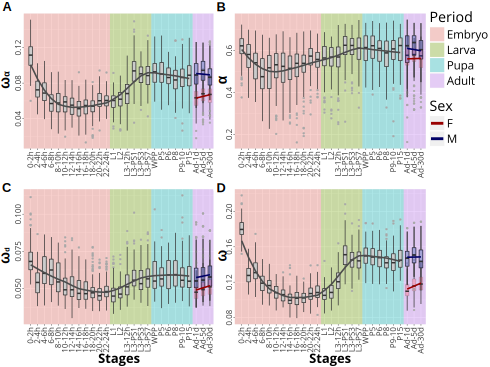
\includegraphics[width=0.9\textwidth]{./Images/Art-IV/OmegaA_lifecycle.png}
  \centering
  \caption{\textbf{ {\large$\omega_{\alpha}$} (A),  {\large$\alpha$} (B), {\large$\omega_{d}$} (C), {\large$\omega$} (D) through the life cycle of \textit{D. melanogaster}} Each time point represents 1,000 random samples of 350 genes (with replacement) expressed in a stage. Red line represents a LOESS regression. Female and male stages are fitted to a linear regression. There are 12 embryonic stages at 2hr intervals (from 0h to 24h). Larval stages at first instar (L1), second instar (L2) and third instar (L3). L3 stages are subdivided into the first 12 hours (L3-12h) and several puff stage (L3-PS1 to L3-PS7). WPP is the white pre-pupae stage. Pupal stages are phanerocephalic pupa, 15h (P5), 25.6 hours pupa (P6), yellow pharate, 50.4 hours (P8), amber eye-pharate, 74.6 hours (P9-10), green meconium pharate, 96 hours (P15). Adult stages are 1, 5 and 30 days after eclosion (Ad-1d, Ad-5d, Ad-30d).
  }
  \label{fig:Art-IV-OmegaA_lifecycle}
\end{figure}
%%%%%%%%%%%%%%%%%%%%%%%%%%%%%%%%%%%%%%%%%%%%%%%%%%%%%%%%

%% result genomic determinants
\subsection{Correlation of adaptation with some genomic determinants}
Many "genomic determinants" temporal profile correlate either positively other negatively with $\omega_{\alpha}$ (IV, Figs 2 and 3). 
%
Thus, messenger complexity (number of transcripts divided by the number of exons) correlates with $\omega_{\alpha}$, whether if comparing males or females (rank correlation; see study IV).
On the contrary, gene size, number of exons, codon usage bias and number of transcripts per gene negatively correlate with $\omega_{\alpha}$, whether if comparing males or females (all with significant rank correlations; see study IV). 

Using a fuzzy clustering algorithm (see study IV), it was found that genes that are expressed at high levels in the earliest development and rapidly decrease their expression to very low levels (cluster 1 and 2; IV, Fig. 4) are likely responsible for the high $\omega_{\alpha}$, $\omega_{d}$, $\omega$ and $alpha$ values in the first embryonic stages (IV, Fig. 4). Also, it was found that a subset of genes whose expression increases only in the last stages of embryonic development (cluster 8; IV, Fig. 4) showed high $\omega_{\alpha}$ and $\omega$.

%Clusters 1 and 8 with high $\omega_{\alpha}$ also showed significantly low gene size, number of exons and number of transcripts (permutation test, p < 0.001).


%
%\textit{D. melanogaster}, as all holometabolous insects, has an indirect development with two active free-roaming phases, the larva and the adult, and two inactive sessile developmental phases, the embryo and the pupa. 
The morphology and other aspects of the phenotype of the larva and the adult arise primarily through the genetic, cellular and tissue interactions of embryonic and pupal development, respectively.
Therefore, adaptation in the larva or the adult morphology should be reflected in adaptation in the genes expressed in embryonic development and pupal development, respectively.

The evidence that most embryonic development shows low rates of adaptive change while the larva and pupa stages show higher rates of adaptative change suggests that there has been more adaptive changes in the adult morphology than in the larva morphology (between \textit{D. melanogaster} and \textit{D. yakuba}). To the extent that those adaptive changes in genes reflect adaptive changes in the phenotype and to the extent that adult morphology in holometabolous insects barely changes after pupation, our results suggest that this adaptation would have occurred both in male and female morphology.

\subsection{Results support the Hourglass model}

The results presented here are consistent with the Hourglass model (HG), specially for the early and mid embryonic development.
%This consistency is, however, rather weak since there are no major differences in ω between embryonic stages after the eight hour. 
During the first 6 hours $\omega$ and $\omega_{\alpha}$ are significantly high (permutation test), which is consistent with the expectations of the HG.
The same parameters are significantly lower during mid-embryogenesis, which is also consistent with the higher conservation expected from the HG.
However, during late embryonic stages (from 10-12h to 22-24h) $\omega$ and $\omega_{\alpha}$ are significantly lower (permutation test), which is not what is expected from the HG.


The phylotypic stage in Drosophila has been suggested to be just between the 6th and 10th hour \citep{Drost2015}.

In contrast with some previous studies \citep{Davis2005,Kalinka2010} we do not find that the later stages of embryonic development are less conserved. 
It was found however, that the cluster composed of genes whose expression is high only in late development (cluster 8; see study IV), shows a significant $\omega$ and $\omega_{\alpha}$. In here, this group of genes have only a minor effect on the global pattern. It could be that, due to the different methodology used by these other studies, these genes would have a relatively higher effect on the pattern observed. it could also be that the differences are partly due to the different species used in the analyses.\citet{Davis2005} use D. pseudoobscura as outgroup species while \citet{Kalinka2010} use six different \textit{Drosophila} species including \textit{D. melanogaster} but not \textit{D. yakuba}, the species used as outgroup in this work.

Despite these differences, the overall $\omega$ and $\omega_{\alpha}$ pattern (Fig \ref{fig:Art-IV-OmegaA_lifecycle}) is consistent with the HG model of embryonic development in \textit{Drosophila} \citep{Kalinka2010}.

\paragraph{Genomic determinants}

In here, we suggest that the temporal patterns of adaptive change and conservation through development may result or be affected by the temporal patterns of change in some of these genomic determinants (gene size, exon and transcript number and intron length) through development. 
These patterns of change in these genomic determinants would simply be a consequence of the complex spatio-temporal regulation of gene expression occurring in embryonic 
development (as suggested many times before on more qualitative grounds \citep{Duboule1998}.
	\clearpage



%%%% -----------------------------------------------------------------
%%%% -----------------------------------------------------------------

\chapter{Concluding Remarks}

The study of organismal complexity during embryonic development presented here shows that there are commonalities and differences between \textit{D. melanogaster} and \textit{C. intestinalis}. Both species showed a non-linear increase in all complexity measures, while the most remarkable difference is the timing of the major change in complexity, which is earlier in \textit{D. melanogaster} (around gastrulation).
Another common pattern is the early increase in complexity when considering only transcription factors or growth factors (or other signalling molecules). This confirms the special role these genes have in early metazoan development. It could be therefore expected that the evidence presented here, regarding these type of genes, should be observed also in other species. 

One important result of this work is that within each species, the three complexity measures showed a similar pattern (even when it would not be necessarily the case; see section X). This means that altogether, these measures (compartmentalization, disparity and roughness) are reflecting a global pattern of increase in complexity in each species. Therefore, it could be hypothesized that a similar increase in complexity would be found using alternative measures of complexity (e.g., spatial entropy). Further analysis would be required to test this hypothesis.
Also, the Synexpression Territories analysis allowed to "reconstruct" the main embryonic differentiation events in both species in a consistent manner with the current knowledge of the development of these model organisms and without focusing in specific genes.

The elaboration of an adaptation map on the fruit fly embryo can be considered a proof of concept of how the combination of diverse fields like evolutionary developmental biology and population genomics, and new techniques such as the phylostratigraphy, can be useful to give a fresh view on an old problem.
Using these maps, it was possible to visually identify that the center (internal part) of the embryo expresses a more conserved and older transcriptome, while the outside (external part) expresses phylogeneticaly younger and less conserved genes. This evidence seems to support the hypothesis of the antecedence of the endoderm with respect to the ectoderm \citep{Hashimshony2014}. It would be interesting to extend this adaptation mapping analysis for the entire development (until the adult stage) as it could be that in later stages, different structures or organs have been under positive or negative selection.

The estimation of adaptation over the entire life cycle of \textit{D. melanogaster}, as presented here, supports the HG model of development. We find, as other analyses previously have, that the mid-embryogenesis is highly conserved. The work presented here is different from previous ones in that it uses a more complete spatio-temporal dataset and a method that uses inter and intra-specific DNA coding variation to estimate, with an unprecedented precision, the proportion of adaptive changes.

Furthermore, as a result of this work is hypothesized that the hourglass model can be partially explained by various genomic features. However, further work is necessary to test this hypothesis.

%In here, I have taken advantage of the great amount of information about developmental gene expression that has accumulated in many years from collective efforts of the developmental biology community. This great amount of accumulated data allows to shift the focus from single genes to a systemic approach in which the global statistical properties of development can be investigated.


OPEN QUESTIONS AND FUTURE DIRECTIONS

The emergence of new techniques, like "spatial transcriptomics" of tissue sections at single-cell resolution \citep{Stahl2016} could make possible to have information, derived from a single experiment, of all the genes expressed in a 2D section of an embryo. The application of the measures presented here could be apply to this kind of data in a straightforward manner, solving the limitation in resolution of the work presented here.

It is important to mention that this work has used differential gene expression in the embryo and its spatial distribution as a tool to investigate complexity. However, embryonic development can not be reduced to differential gene expression. Cellular behaviours and the physical properties of the cells and tissues have also a causal role in the developmental process. It would be interesting to be able to measure the differential apportionment to complexity increase of the different developmental mechanisms.


The increase of organismal complexity and the study of adaptation during development remain fascinating topics after many centuries, and still offer many open questions to be solved. The incredibly fast pace of data generation, the development of new techniques and sophisticated methods give hope to finally open the black box of development.

%%%%%% for results of compartmentalization
%
%It could be expected that these early increase in complexity in drosophila is shared by all insects with a syncitial blastoderm stage. It could be that there are differences between these based on the number of cell divisions until the blastoderm is cellularized. It is known that Drosophila cellularizes relatively late (so there is more time for patterning within the syncitial bastoderm). In contrast, the desert locust (Schistocerca gregaria) cellularization occurs very early, before the formation of the blastoderm (REF Ho).
%
%The rapid development in drosophila could be due to selective pressures on the time of development, caused by the the eggs being layed ephemeral resources such as decaying fruits (this classical view has been chalenged recently; reviewed in REF Prasad). 
%The embryonic development of D. melanogaster takes around 1 day at 22 degrees. Even when developmental time can vary in a three fold manner depending on the Drosophila species and temperature (D. virilis embryonic development at 18 C takes more than 45 hours, compared to less tha 15 hours at 30 C in D. ananassae: REF Kuntz), it can be considered fast compared the dessert locust. In the locust, embryonic development takes around two weeks in calid environments in West Africa but it can take up to 70 days in the cooler temperatures of North Africa (REF locushanbbook).
%
%Also, it would be interesting to know if there are some differences between the two main modes of segmentation in insects, i.e., short germband and long germband. The red bettle (Tribolium castaneum) is most popular short germband inset that serves as a developmental biology model organism. Many valuable resources have become available in the last decades/years (REF Bucher). 
%
%
%The period of egg development, between laying and hatching, is called the incubation period. The rate at which eggs develop varies according to the soil temperature. For example, in the summer breeding areas of West Africa, the Red Sea coast and lowland India the incubation period takes 10-14 days but this is extended to 25-30 days in the cooler spring breeding areas of central Arabia, southern Iran and Pakistan while in North Africa it can take as long as 70 days in exceptionally cold weather

\clearpage
%%%% -----------------------------------------------------------------
%%%% -----------------------------------------------------------------

%\listoffigures
%\printnomenclature
%%%% -----------------------------------------------------------------
%%%% -----------------------------------------------------------------
%\bibliographystyle{plain}

%%%%% The bibliography is written in a small fontsize and in 2 columns
\begin{multicols}{2}
{\footnotesize
\bibliography{Bibliography}
}
\end{multicols}

%%%% -----------------------------------------------------------------
%%%% -----------------------------------------------------------------
\end{document}